
\documentclass[a4paper,11pt,linenumbers]{article}
\pdfoutput=1 % if your are submitting a pdflatex (i.e. if you have
             % images in pdf, png or jpg format)
%\usepackage{amsfonts}
\usepackage{color}
\usepackage{placeins} % floatbarrier definition
\usepackage{graphicx}
\usepackage[perpage]{footmisc}
\usepackage[normalem]{ulem}
\usepackage{caption}
\usepackage{subcaption}
\usepackage{jinstpub} % for details on the use of the package, please
                     % see the JINST-author-manual
\usepackage{lineno}

\newcommand{\RanComment}[1]{\textcolor{green}{#1}}
\usepackage{soul}                     
\newcommand{\mmd}[1]{\textcolor{blue}{#1}}
\makeatother


\title{Directional Xenon Measurement }
\linenumbers


%% %simple case: 2 authors, same institution
%% \author{A. Uthor}
%% \author{and A. Nother Author}
%% \affiliation{Institution,\\Address, Country}

%% more complex case: 4 authors, 3 institutions, 2 footnotes
%\author[a,b,1]{F. Irst,\note{Corresponding author.}}
%\author[c]{S. Econd,}
%\author[a,2]{T. Hird\note{Also at Some University.}}
%\author[c,2]{and Fourth}
%
%% The "\note" macro will give a warning: "Ignoring empty anchor..."
%% you can safely ignore it.
%
%\affiliation[a]{One University,\\some-street, Country}
%\affiliation[b]{Another University,\\different-address, Country}
%\affiliation[c]{A School for Advanced Studies,\\some-location, Country}
%
%% e-mail addresses: only for the Corresponding author
%\emailAdd{first@one.univ}
%
%
%

\abstract{Abstract...}



\keywords{Only keywords from JINST's keywords list please}


\arxivnumber{1234.56789} % only if you have one
\begin{document}
\maketitle
\flushbottom
\section{Introduction}
\label{sec:Intro}

The use of Noble-liquid detectors in the field of astroparticle physics has increased in the past decades. Detectors aiming at measuring Dark Matter (DM) particles and neutrinos properties use large liquid argon or liquid xenon (LXe) chambers~\cite{Aprile:2009dv,Rubbia:2013tpa}. Current and future experiment for DM detectioin are tuned to detect weakly interacting massive particles (WIMPs), a postulated candiadte for DM particle~\cite{Bertone:2010zza}. LXe based detectors are to date the leading in sensitivity and size for these searches~\cite{Aprile:2017iyp,Akerib:2016vxi,Fu:2016ega,Aalbers:2016jon}. 

When a particle interacts within the LXe media, it forms a cloud of excited and ionized states with typical length of 100~nm. The excited Xe ($Xe^*$) combines with other Xe atoms to form an excited dimer state (excimer) when they decay to ground state they emit light. 
\begin{equation} \label{eq:XeSci1}
 Xe^*+Xe \rightarrow Xe^*_2 \rightarrow 2Xe + h \nu , 
\end{equation}
The electrons emitted from the ionization can recombine with a surrounding atom, this process of recombination provides another possibility to produce excimers,
\begin{equation} \label{eq:XeSci2}
\begin{split}
  &Xe^{+} + Xe \rightarrow Xe^{+}_2 \\
  &Xe^{+}_2 + e^{-}  \rightarrow Xe^{**} \\
  &Xe^{**}   \rightarrow Xe^* + heat .\\
  \end{split}
\end{equation}  
Once $Xe^*$ is produced it adds to the scintillation process explained in~\ref{eq:XeSci1}. There are two types of $Xe^*_2$ excimer states, singlet and triplet, with lifetime of $\sim3$ ns and $\sim25$ ns respectively. The wavelength emitted by these states is between (175-180)~nm which is lower then the lowest excitation of xenon, and therefore travel through it to reach a photo-detector situated outside the LXe. Although much is measured on these scintillation processes, the basic knowledge of the quantum properties of these interactions is based on experiments preformed several decades ago.

The phenomenon of supperradiance in which identical quantum states ``communicate" through electromagnetic field if in close proximity, is well studied. In certain conditions the emission of photons from these correlated states is very different then the sum of random states. This difference is in spectral, temporal and spatial properties~\cite{DickeSR,GROSS1982301}. Early studies show that scintillation in LXe can produce coherent amplification of light~\cite{BasovSRTheory,MiesSRExp}. These studies were focusing on the macroscopic ionization using high energy density electron beams. 

The understanding and quantification of the microscopic effects of non linear phenomena such as supperradiance in Lxe for a single interaction, can improve DM experiments to reduce background by the extra knowledge of directionality. irreducible background such as coherent neutrino nucleus scattering of neutrinos from the sun can be discard.

In this paper we present an experimental set-up called DIREXENO (Dirextional Xenon) aiming at measuring the spatial distribution of LXe scintillation light, and quantify non-isotropic emission.   
\section{Experimental Setup}
\label{expSetup}

%%%%%%%%%%%%%%%%%%%%%%%%%%%%%%%%%%%%%%%%%%%%%%%%%%%%%%%%%%%%%%%%%%%%%%%%%%%%%%%%%%%%%%%%%%%%%%%%%%%%%%%%%%%%%%%
%Initiator: Ran Itay
%Last modified by: MM Devi, May 26 2017
%Comment: The detector section has been modified. MMdevi's changes are made in blue
%%%%%%%%%%%%%%%%%%%%%%%%%%%%%%%%%%%%%%%%%%%%%%%%%%%%%%%%%%%%%%%%%%%%%%%%%%%%%%%%%%%%%%%%%%%%%%%%%%%%%%%%%%%%%%%

The experimental setup that is described in this section, is designed to measure, the spatial and \RanComment{temporal (I think there is a better way to say it)} properties of LXe scintillation. However it is designed in a modular way, so it can serve different requirements from different future experiments. 
There are four main building blocks constructing the full setup, The gas handling system, the cryogenic system, the detector system, and the data acquisition (DAQ) system. Each building block can be replaced without effecting the others. The full assembly 
(figure.~\ref{fig:fulldet}) is held on three separate wracks, one for the DAQ, while the two others hold the cryogenic detector and gas handling system are joined using a 100mm bar with shock absorbers on both sides. Some of the guidelines for the design of DIREXENO is based on~\cite{Giboni}  

\begin{figure}[t!]
\centerline{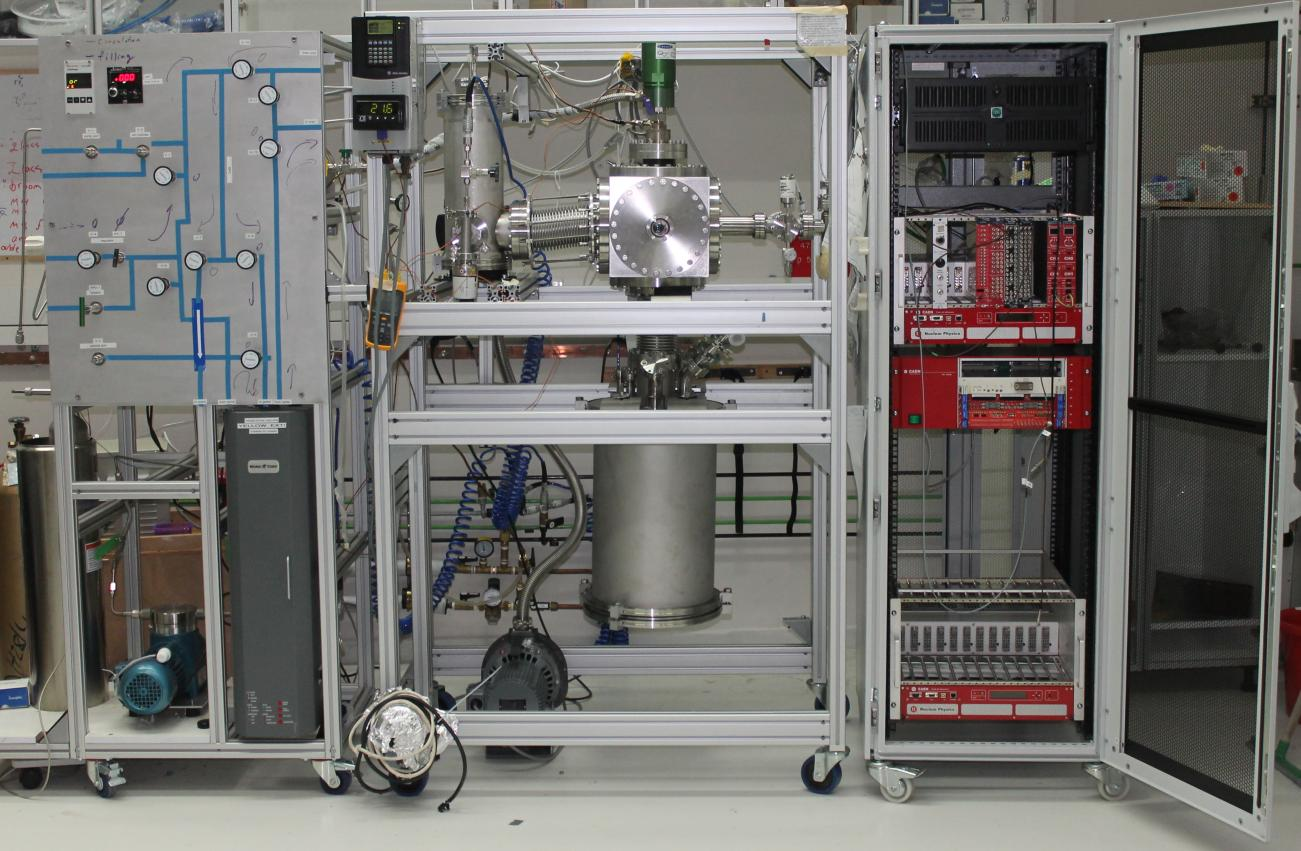
\includegraphics[width=1.\linewidth]{FullDet.jpg}}
\caption{DIREXENO. On the left the purification system, in the middle the cryogenic and detector chamber, and on th right the Data acquisition system.}
\label{fig:fulldet}
\end{figure}

\subsection{Gas handling system}
\label{subsec:gas}

A typical LXe detector must keep a high level of purity. Careful selection and meticulously cleaning of all parts before mounting, 
is needed, however is not sufficient. The desired level of most detectors of impurity concentration is at the level of 1 ppb $O_2$ 
equivalent~\cite{Aprile:2009dv}. This is crucial to allow ionization electrons drift for several cm. To reach that level in a 
reasonable amount of time (several days instead of months), continuous purification is needed. The gas handling system, provides this process, 
alongside with all gas handling operations such as filling and recuperation.

During purification mode, xenon is taken from the chamber (in liquid phase)
passes through a heat exchanger\footnote{GEA GBS100M-24 plate heat exchanger} where it is heated and vapored. The xenon is forced 
by a KNF diaphragm pump into a hot getter\footnote{MONO-TORR
PS4-MT15-R-2} which cleans the xenon from most impurities. The xenon
also passes through an MKS Mass Flow Controller\footnote{MKS mass flow controller} (MFC), this allows monitoring and controlling the amount of xenon in the system. 

After the xenon is purified, it is delivered back to the cryogenic system through the heat exchanger, there the remained xenon gas is 
liquefied before it continuous back to the chamber. A schematic of this system is shown in fig.~\ref{fig:gasSchematic}.


\begin{figure}[t!]
\centerline{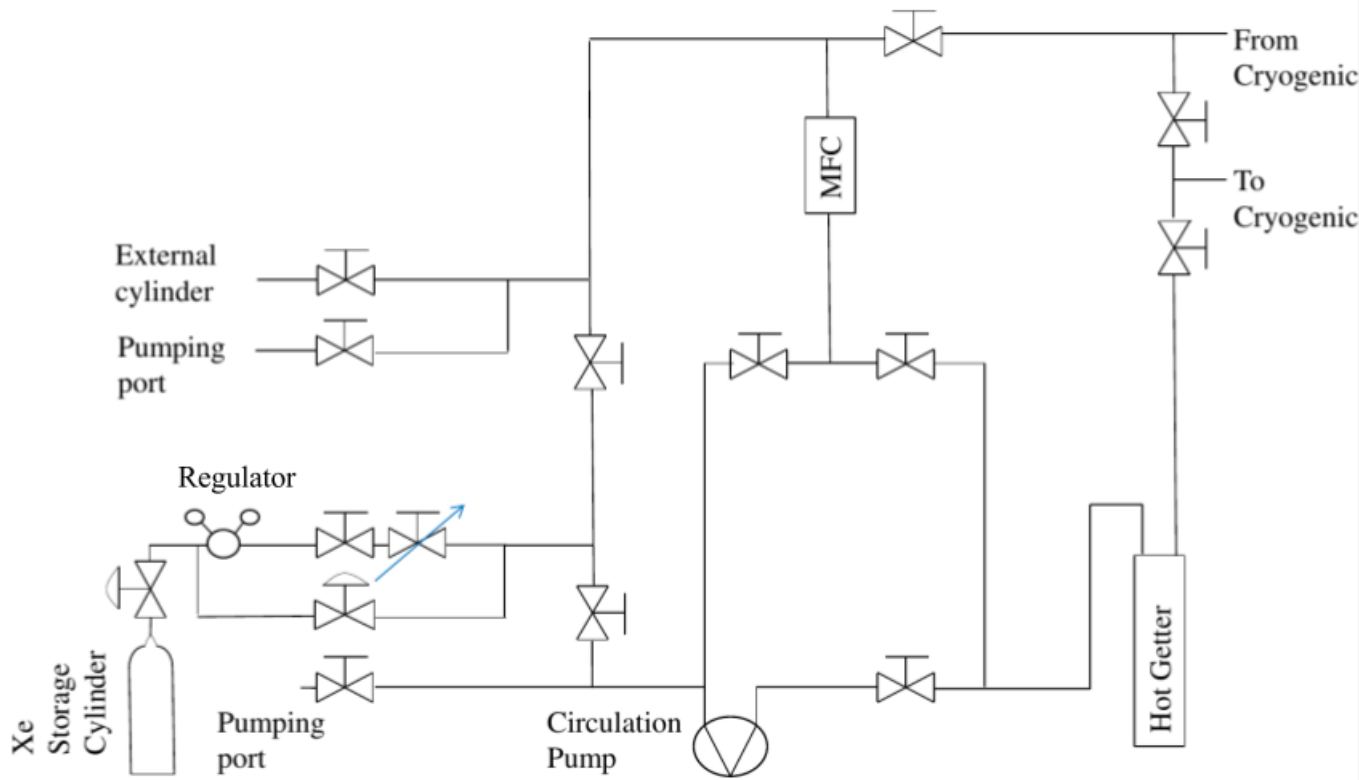
\includegraphics[width=1.\linewidth]{GasSchematics.png}}
\caption{Schematics of the purification system. High pressure valves are indicated as valves with arcs. Needle valves are indicated as 
a valve with an arrow.}
\label{fig:gasSchematic}
\end{figure}

\subsection{Cryogenic system}
\label{subsec:cryo}

Remote cooling is generally used in DM experiments due to background radiating from the cooler to the detector. Although in our system 
this is not of great importance there are still several advantages to remote cooling such as: lowering acoustic noise from the cryo-cooler 
and flexibility to design changes. The cryogenic system is connected on one side to the gas system and on the other to the detector chamber, 
any change in the system (e.g, cooler type or model) requires the change of that specific part without changing the detector nor the gas system.

The system is made out of two chambers, the outer vessel (OV) which holds the insulation vacuum, and the inner vessel (IV) that holds the 
xenon. In addition to the vacuum which prevents heat leaks from diffusion and convection, the entire IV is covered by multi layer aluminized 
Myler to prevent heating via radiation an image of the detector and the CAD design are shown in Fig~\ref{fig:cryo}. 
\begin{figure}
   \centering
    \begin{subfigure}[b]{0.25\textheight}
    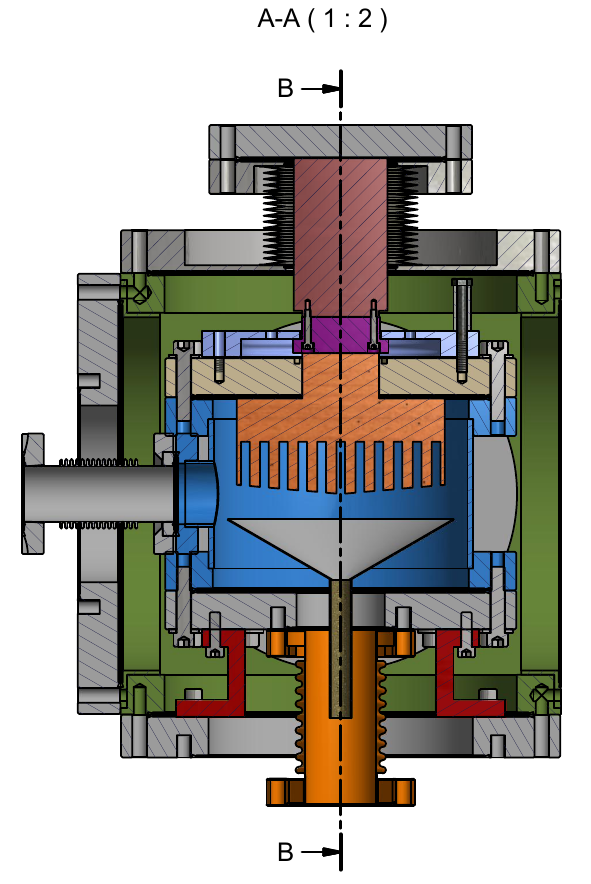
\includegraphics[width=\textwidth]{cryogenic1.png}
    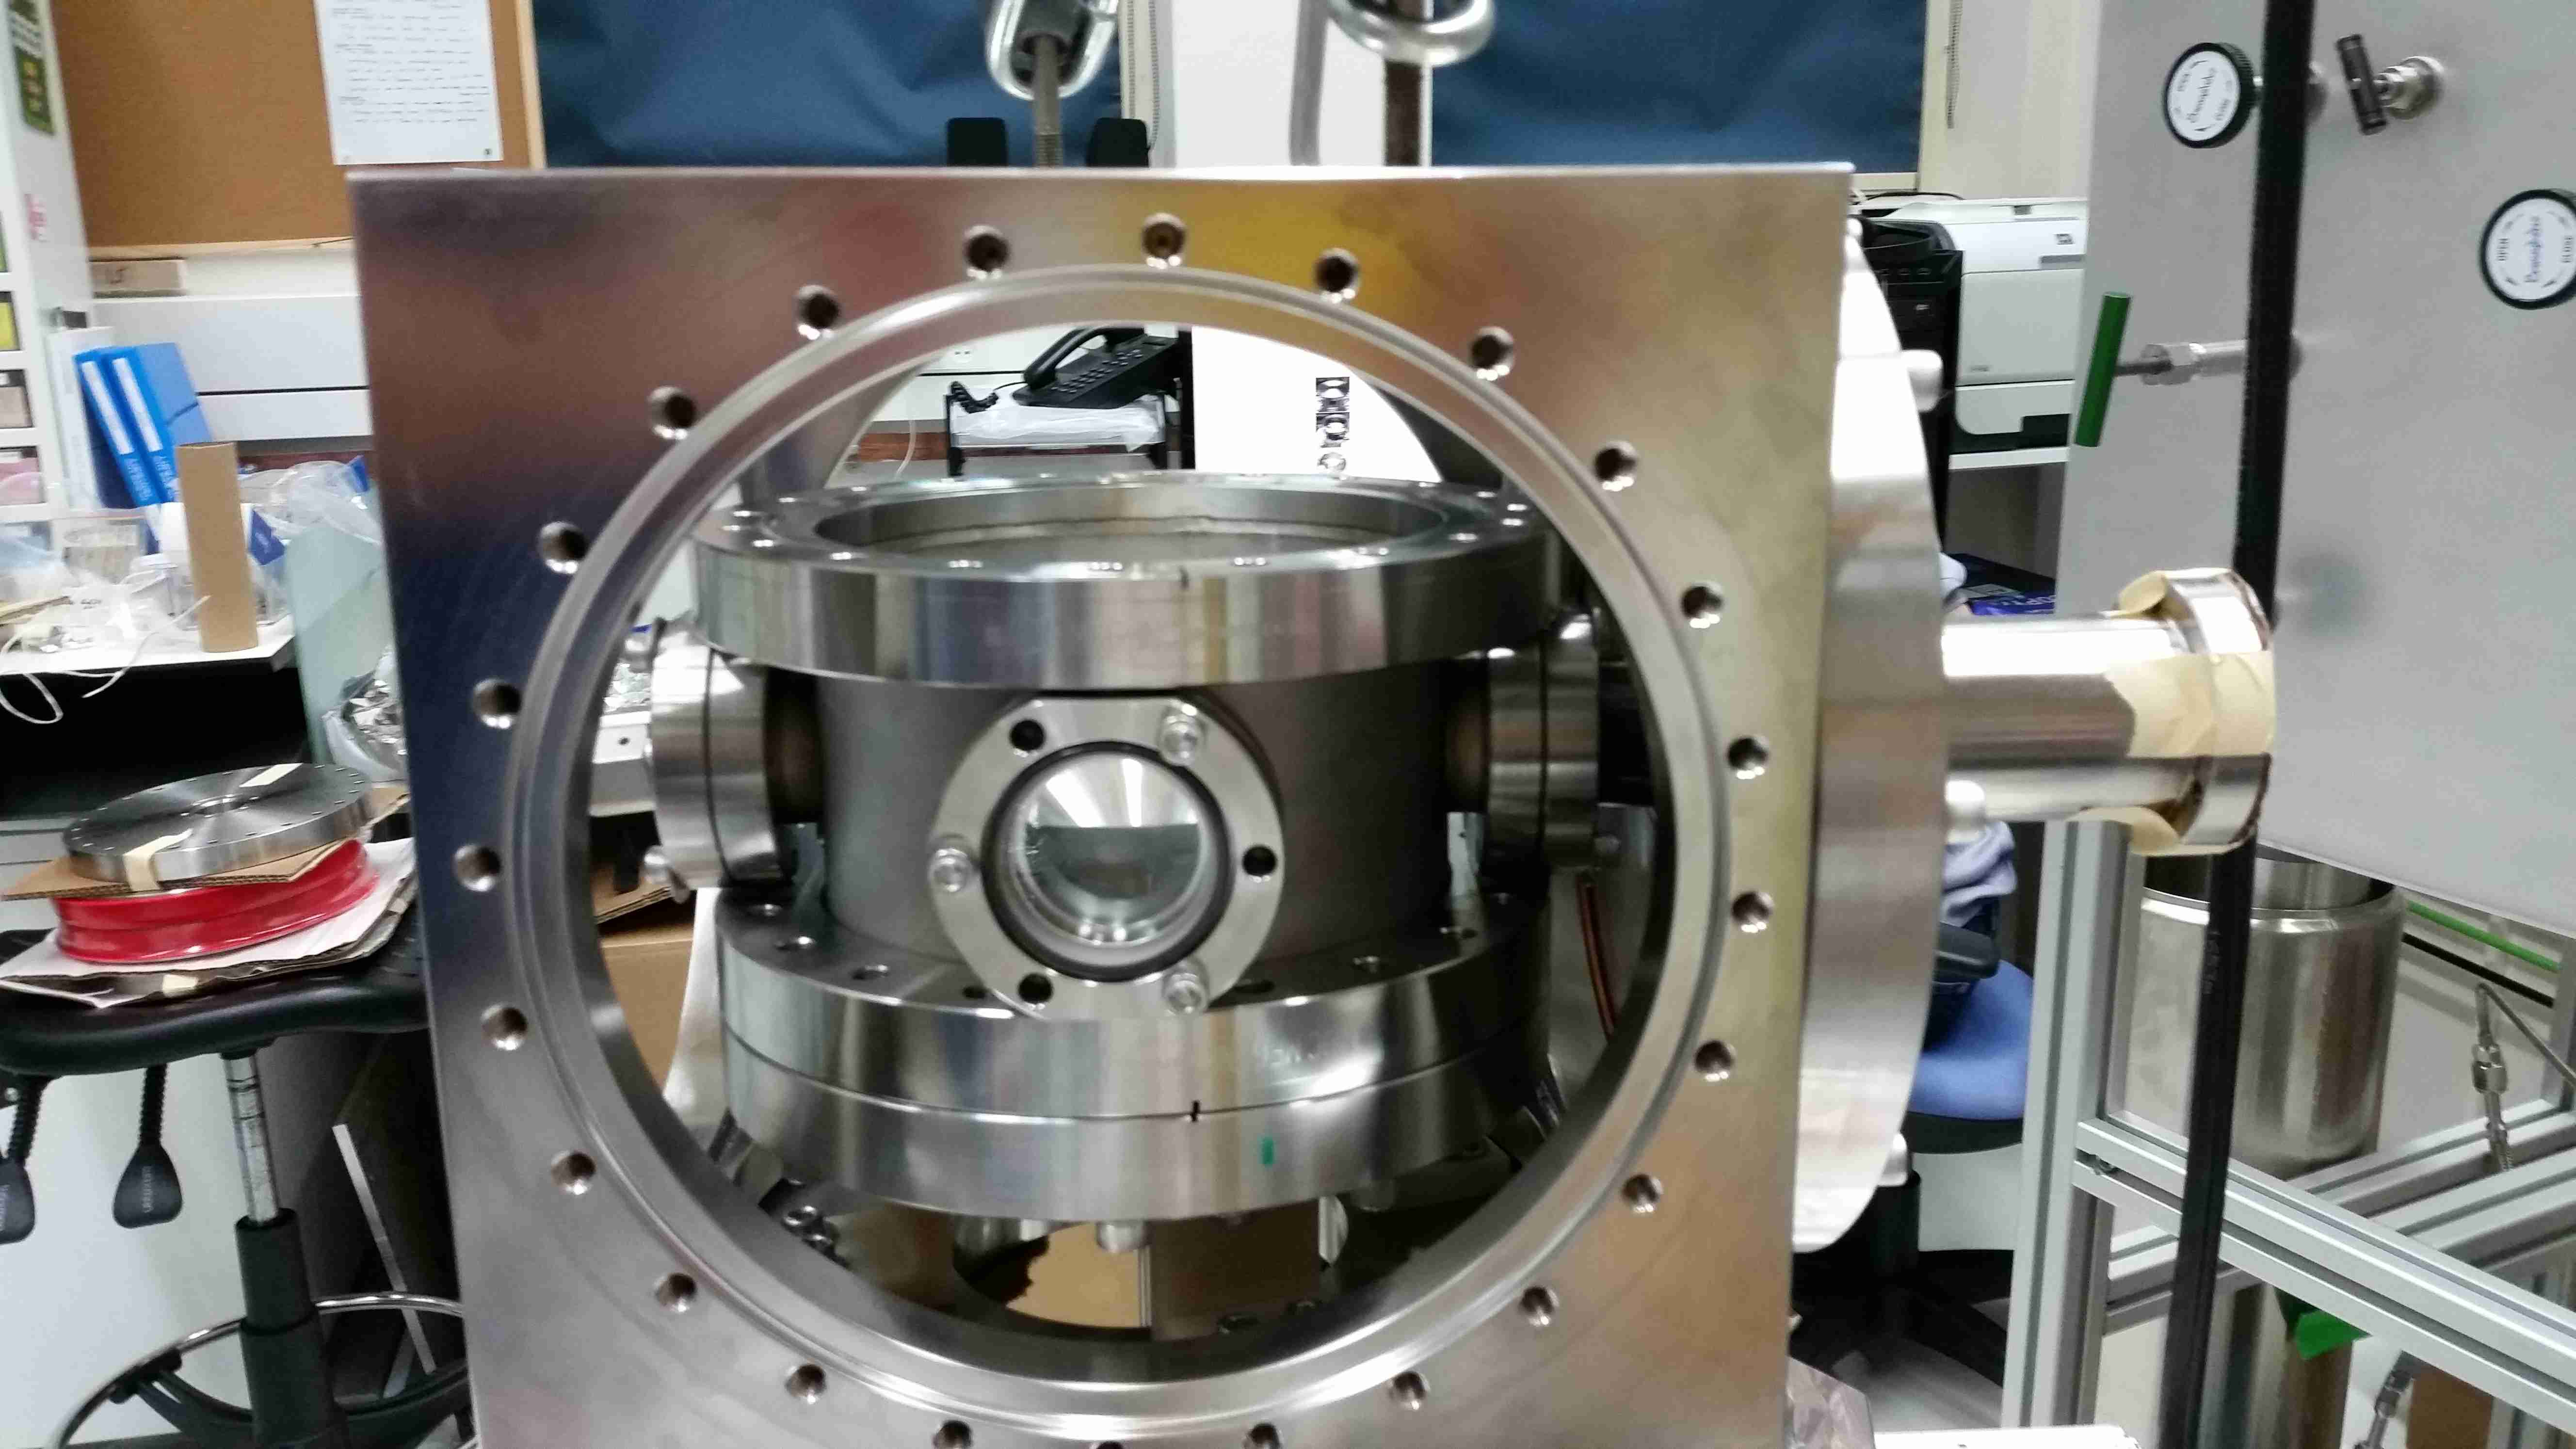
\includegraphics[width=\textwidth]{CryoOpen_small.jpg}
    \end{subfigure}
        \caption{(Top) CAD view of the cryogenic system. (Bottom) Pictue of the cryogenic system. \label{fig:cryo}}
\end{figure}


The OV is made of a 10" CF cube, with ports on all six faces (e.g., FT, pumping ports, view ports). This vacuum is shared with the detector one via a 6" CF flexible bellows.

The IV is made of 1.5" height cylinder with 6" CF flanges on the top and bottom parts of it, and it holds inside xenon. A 120~\,mm diameter cold finger is welded to the top flange of the IV. The design of the cold finger is similar to the design of~\cite{xe100_instr2012}, the inner 
part of the cold finger is made of long fins, therefore the surface area of it is bigger resulting in a better heat transport. The upper 
part of the cold finger is in thermal contact with the cryo-cooler~\footnote{QDrive 20BB 9p6 A 3 AYNBNCO} via a cooper adapter. The copper 
adapter holds two $100\Omega$ pt resistor which are connected to a PID reader\footnote{cryo-con model 18i Cryogenic Temp Monitor} for 
temperature measurements. A Cartridge-heater is also inserted to the copper adapter for emergency heating. 

The cryo-cooler provides up to 70 W of cooling power, and is connected via a $4\frac{1}{2}$" flange to the OV top flange, and reaching the IV top flange. 
Common cryo-coolers used for xenon experiments, work in maximal cooling mode permanently. The QDrive, instead, has temperature control allowing 
it vary the cooling power, which enables to set the temperature with fluctuations smaller then $0.1~\mathrm{C^{\circ}}$ on the cooler itself.

On the inner side of the bottom flange of the IV a thin SS funnel is installed collecting all LXe drops from the cold finger, and delivering 
them to the  detector part. This flange is connected to the detector part, via a $3\frac{3}{8}$" flexible bellows. This bellows hosts two small pipes 
connected to the circulation system, and a third pipe coming from the funnel, all three pipes deliver LXe whereas the GXe is filling the bellows. The separation between the LXe coming from the gas handling system (clean) and the LXe coming from the cold finger (more dirty) allows the filling of clean LXe to different parts of the detector. 
%%%%%%%%%%%%%%%%%%%%%%%%%%%%%%%%%%%%%%%%%%%%%%%%%%%%%%%%%%%%%%%%%%%%%%%%%%%%%%%%%%%%%%%%%%%%%%%%%%%%%%%%%%%%%%%%%%%%%%%%%%%%%%%%%%%%%%%%%%%%%%%%%%%%%%%%%%%%%
\subsection{The Detector}
\label{subsec:det}
 

\mmd{The detector refers to the chamber and its inner assembly that contains the liquid Xenon bubble, the photomultiplier detectors 
around it and their accessories. This chamber is placed below 
the cryogenic system.}
\sout{The Detector part refers to the whole apparatus below the cryogenic system.} 
\RanComment{This needs to be changed so it will be written in sec. describe bla and in sec .. describe blabla, it is bad practice to say in the next two subsec, as this can be changed in the future.} \mmd{We describe the detector chamber and its interface to the cryogenic system in section \ref{subsubsec:detchamber}. In the two 
subsequent sections we discuss the optical assembly that holds the liquid Xenon and the Photomultiplier detectors.}

%%%%%%%%%%%%%%%%%%%%%%%%%%%%%%%%%%%%%%%%%%%%%%%%%%%%%%%%%%%%%%%%%%%%%%%%%%%%%%%%%%%%%%%%%%%%%%%%%%%%%%%%
\subsubsection{\mmd{The detector chamber and its interface to the cryogenic system}}
\label{subsubsec:detchamber}

The \RanComment{detector} chamber is built such that apart from the interface to the cryogenic system, it can be changed and modified easily for future experiments.
The interface unit is built out of 2 flanges welded together via 7 tubes, which serve as service ports for electrical and other feedthroughs. 
The upper flange, ISO-K NW320, is part of the OV and shares the insulation vacuum of the cryogenic system, the bottom one , CF-8", is 
part of an IV for future detectors, and would hold xenon inside. For our experiment we modified the CF flange to fit also a $4\frac{5}{8}$" CF 
flange which we use.

The OV is closed with a cylinder XXX~\,cm height closed from the bottom with another ISO-K NW320 flange, the height of the cylinder is determined 
such that the maximal height of the whole apparatus is 190~\,cm, allowing the mobility of the detector through standard doors.
 
The $4\frac{5}{8}$" CF flange is connected to a closed vessel internally divided into two parts. This vessel serves as a xenon reservoir. The two parts of the vessel are connected to a spherical orb from above (inner part) and from below (outer part). LXe is circulated such that new LXe drips into 
the outer part and pumped from the inner one. This way the liquid level is controlled, and the sphere itself is always filled with LXe. 

\RanComment{I think this part should be deleted as it is explained after.The main part of the detector is the spherical orb, which is made of fused silica. In the center of it, a smaller sphere is curved to hold the 
LXe, two invar pipes are connected to it from the top and bottom with SS mini-CF flanges at the end, to circulate the xenon (see Fig.~\ref{fig:sphere}). 
The sphere stands in the center of 20 PMTs\footnote{r8520-406 Hamamatsu 1" PMT} to detect light emitted from the LXe.}

\RanComment{The bottom flange of the sphere is held using a brass holder to prevent force or torque applied on the sphere while mounting the detector. The 
brass holder is connected to a plate held from the top 8" flange, and is also used to align this plate at first installation. }

%%%%%%%%%%%%%%%%%%%%%%%%%%%%%%%%%%%%%%%%%%%%%%%%%%%%%%%%%%%%%%%%%%%%%%%%%%%%%%%%%%%%%%%%%%%%%%%%%%%%%%%%%%%%%%%%%%%%%%%
\subsubsection{\mmd{The HPFS Shell to contain LXe}}
\label{subsubsec:sphere}
\RanComment{missing general explanation about the sphere might be that the part I suggested to delete before should go here.}
The LXe target bubble should not be too large in order to avoid double scatters. A spherical shell made of high purity fused silica 
with high transmittance is designed to hold the LXe target. This shell should be large enough to reduce internal reflections, but not too large which would 
attenuate the scintillation light. \sout{Also} The material of the shell should have a refractive index similar to LXe in order to have minimal \RanComment{diffraction when photons from the LXe, move travel from LXe to the sphere and saving the original \sout{change in} the original direction of the LXe scintillation} \sout{ photons coming from the target}. 

\RanComment{I think there is no point saying that according to the factshit ... we should state that we measured it, maybe indicate that our result are consistent with data from supplier (not even sure this is needed.) }We chose corning HPFS 8655 as the shell material. According to the factsheet, the refractive index of HPFS 8655 is 1.575 at 185 nm (LXe R.I. 1.61) and the transmittance 99.8\%/cm at 175 nm. In Fig.~\ref{fig:hpfsRIcalibration}, \sout{we show} \RanComment{are} the refractive indices at various wavelegths as given by the HPFS factsheet and also a naive extrapolation at lower wavelengths which are relevant to us.

\begin{figure}
   \centering
   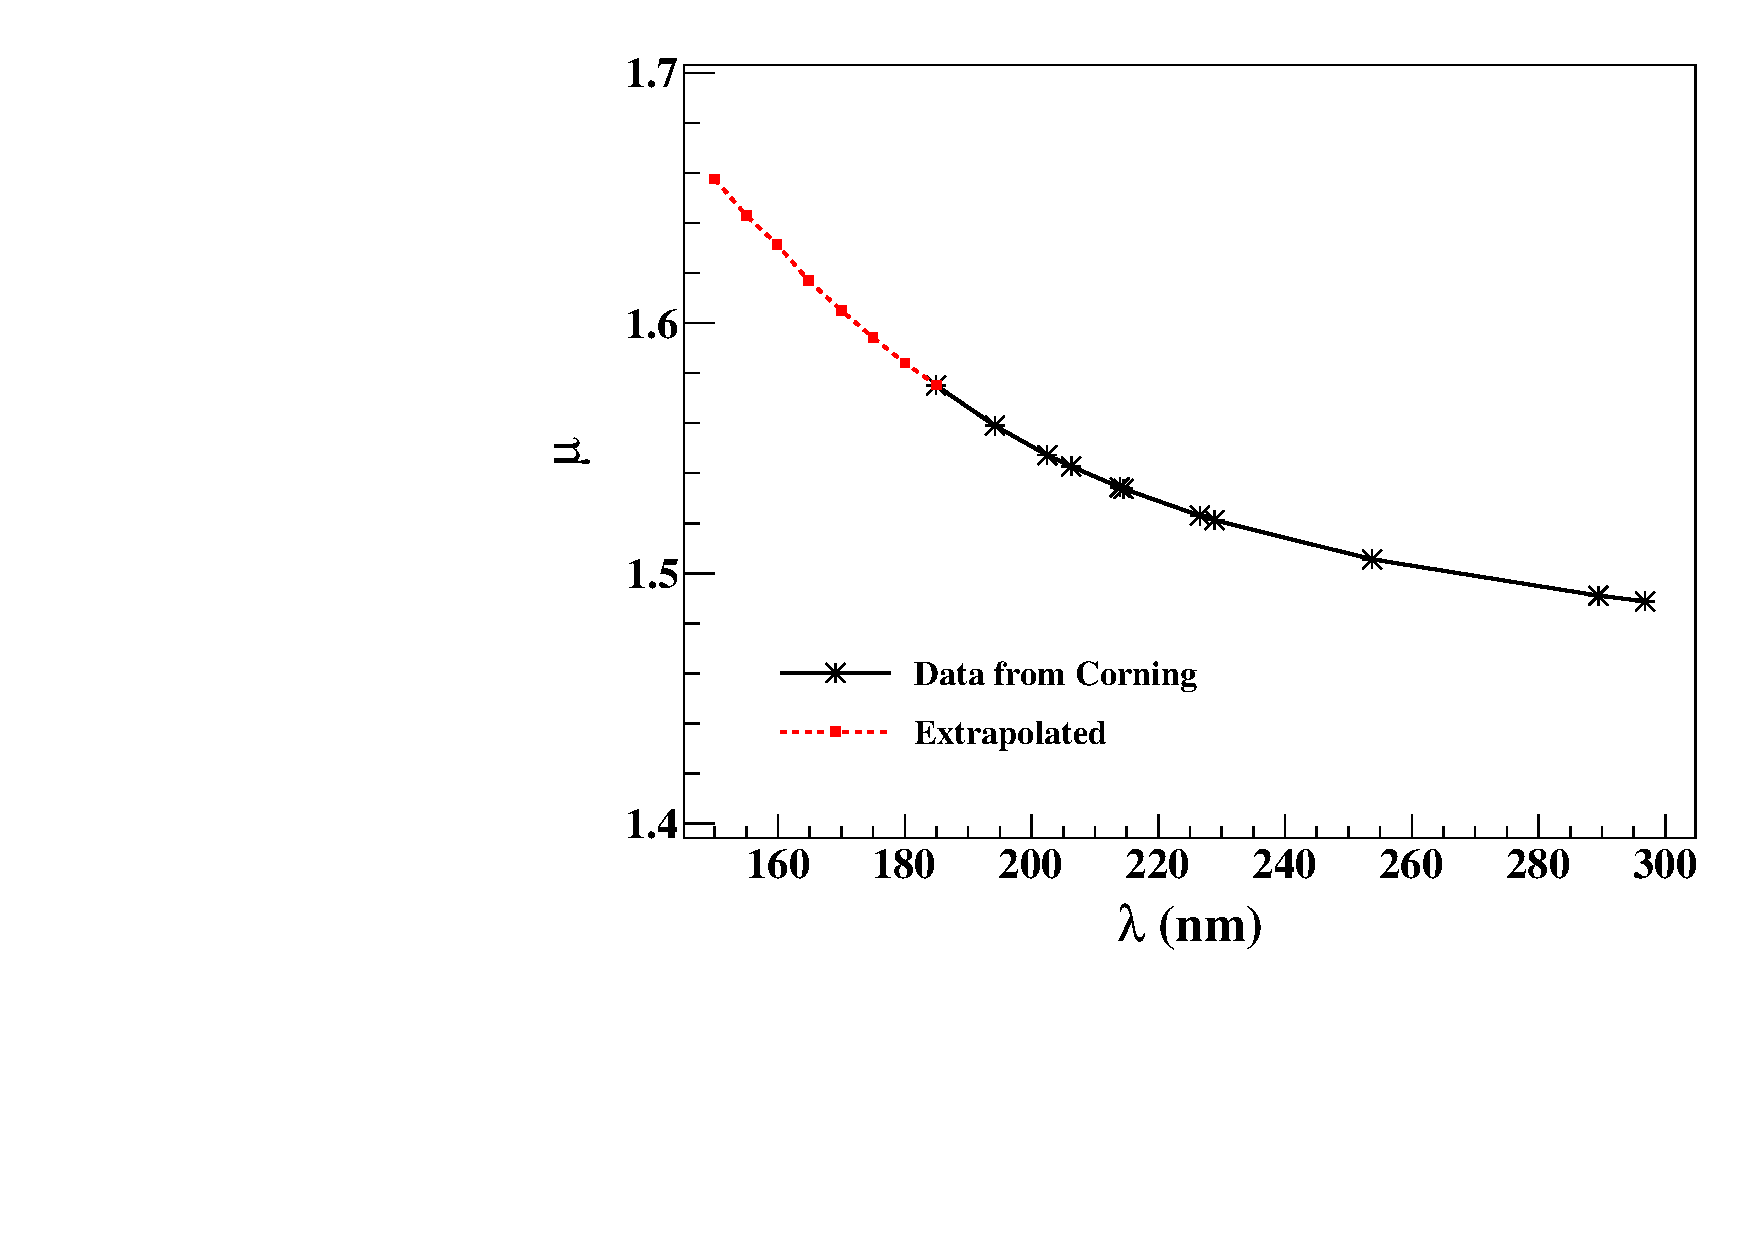
\includegraphics[width=0.8\textwidth]{RI-calibration.pdf}
   \caption{The refaractive indices of HPFS 8655 at various wavelengths. (Top) The values provided from Corning factsheet.
   (Bottom) The values extrapolated at lower wavelengths.} 
   \label{fig:hpfsRIcalibration}
\end{figure}

The transmittance of the material is extremely crucial for us to optimize the dimension of the fused silica shell. Therefore, we obtained a 6 mm thick sample of HPFS 8655 and performed a transmittance testing a VUV monochromator setup. 
A deuterium light source was used to generate a spectrum in
the range (110 - 950)~\,nm, peaked approximately at 160~\,nm. The window of the light source faced a vacuum space pumped to below $10^{-4}$ Torr. The monochromator allows to select the desired wavelengths using a manually rotatable holographic diffraction grating. A PMT placed
in the vacuum measured the intensity of light emitted from the monochromator, with and without the fused silica sample. The ratio of measured intensities was used to calculate the transmittance of the material. In fig.~\ref{fig:transmittance} is the measured transmittances/ 6 mm at 
(150 - 215)~\,nm. At 175~\,nm the sample shows approximately 90\%/6mm measured transmittance which corresponds to an intrinsic transmittance of about 98\%.  

\begin{figure}
   \centering
   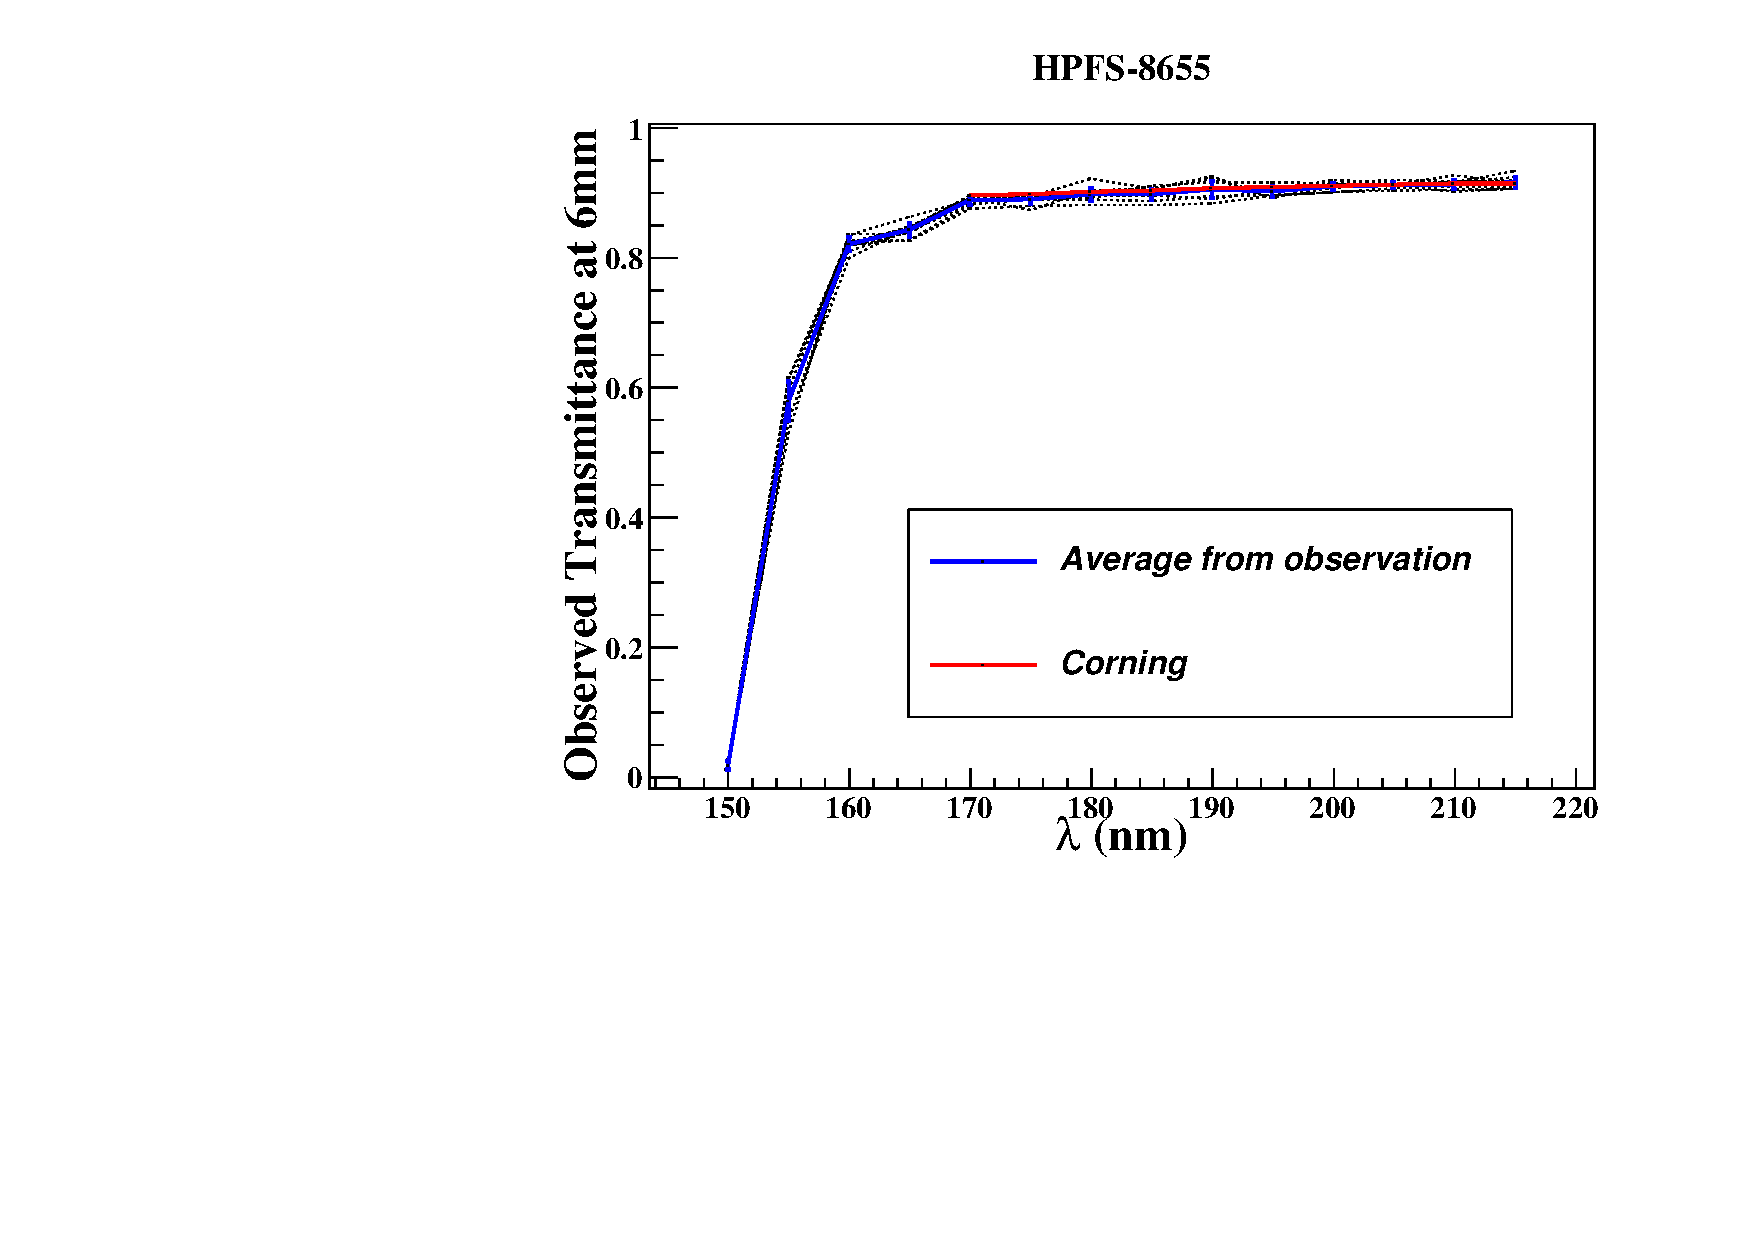
\includegraphics[width=0.6\textwidth]{ObservedTransmittance1.pdf}
   \caption{The transmittance of a 6 mm thick HPFS 8655 sample.} 
   \label{fig:transmittance}
\end{figure}

The dimension of the fused silica shell is optimized by studying the path of the scintillation photons using a GEANT4 based simulation~\cite{AGOSTINELLI2003250}. 
The sources that will be used for exciting the xenon, and creating the supperradiance (signal) as well as the standard emission (background), 
will be $^{137} \mathrm{Cs}$ (662 keV) and $^{57} \mathrm{Co}$(122keV \& 136 keV) for ER and $^{241}$AmBe , D-D neutron generator, or neutron 
produced in an accelerator for NR . The mean free path for this energy is a couple of mm ($^{57} \mathrm{Co}$) and (0.5 - 3) cm ($^{137} Cs$).  
We discuss the simulation in detail in section~\ref{sec:simulation}. 
The outer radius of the shell is 3 cm, while the inner radius of the hollow space that will hold the 
LXe is 1 cm. The flow of the LXe will be maintained by two invar tubes. This shell--system, \sout{as} \RanComment{is} shown 
in Fig.~\ref{fig:sphere} \sout{is being manufactured industrially as par the specification provided by us.}

\begin{figure}
   \centering
   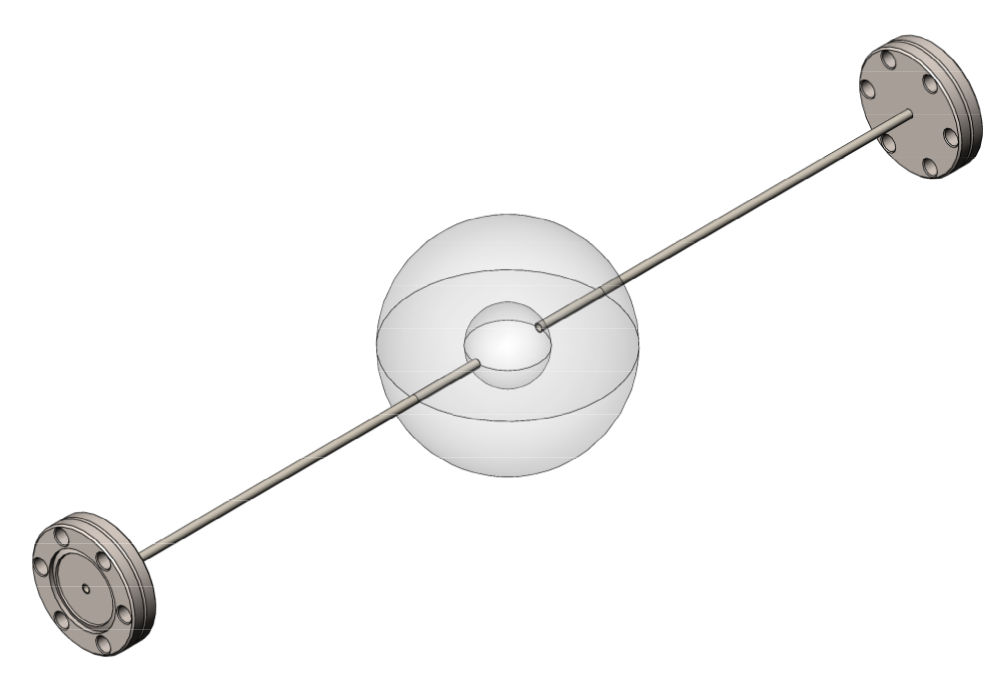
\includegraphics[width=0.6\textwidth]{sphere.png}
   \caption{The technical scheme of the HPFS shell with invar tubing and flanges.} 
   \label{fig:sphere}
\end{figure}


The photons coming out of the system will be detected by twenty 1'' square Hamamatsu R8520-406 photomultiplier 
tubes with an active area of 20.5 mm $\times$ 20.5 mm each. We pick PMTs with a minimum quantum efficiency of 30\% 
at 178 nm. For an applied voltage of 900 V the gain of these PMTs are ~ 2 $\times$ 10$^6$. We use a positive 
voltage divider, also manufactured by Hamamatsu, to provide high voltage to the PMTs.
These 20 PMTs are held with a special aluminum holder, coated with anti-reflection substance. The holder is made of two hemispheres hosting the PMTs in 
3 rows all of them pointing to the center of the fused-silica sphere. the PMTs are held only via their voltage--divider bases. The bases are held using M2 PEEK screws. 
In Fig.~\ref{fig:pmtholder}, one of the holder--hemispheres with the PMTs are shown.

\begin{figure}
   \centering
   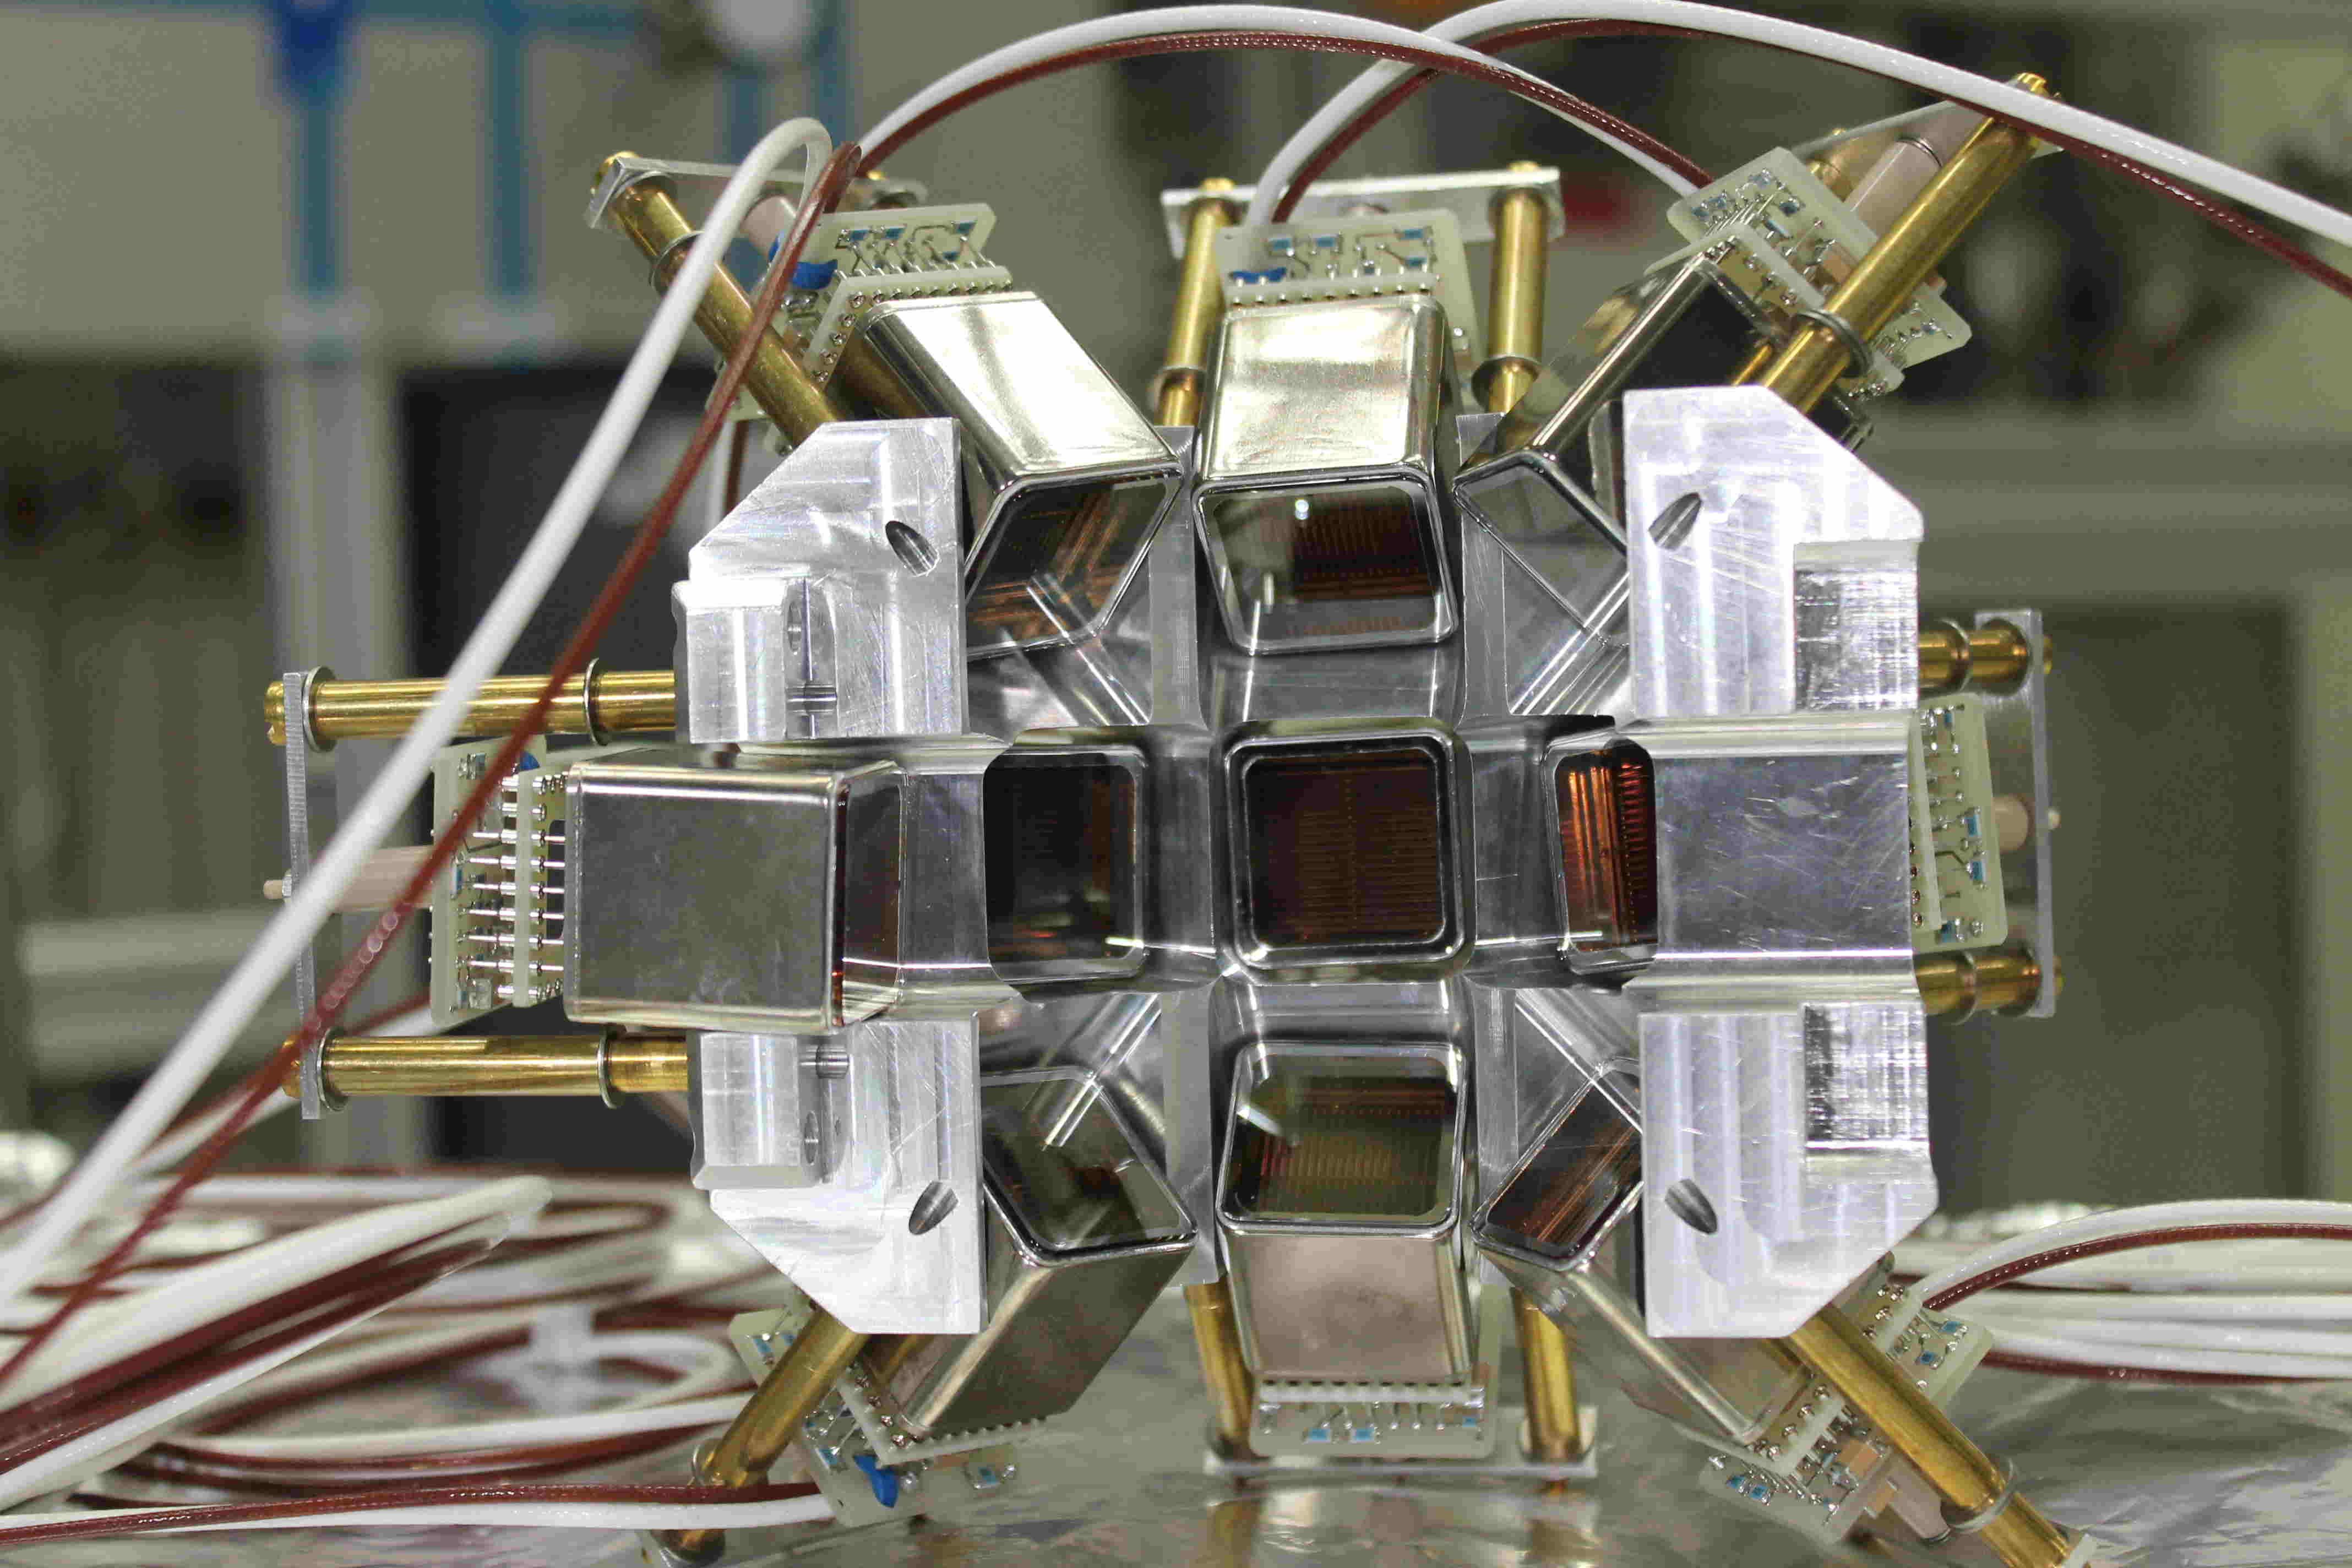
\includegraphics[width=0.6\textwidth]{PMTholder.JPG}
   \caption{A PMT holder--hemisphere. We use two such components to hold 20 PMTS around the target.} 
   \label{fig:pmtholder}
\end{figure}


%\clearpage %temporary MMD
In Fig.~\ref{fig:detector} we present a CAD schematic as well as a real view of the detector part.

%%%%%%%%%%%%%%%%%%%%%%%%%%%%%%%%%%%%%%%%%%%%%%%%%%%%%%%%%%%%%%%%%%%%%%%%%%
\begin{figure}
	\centering
    \begin{subfigure}[b]{0.45\textwidth}
		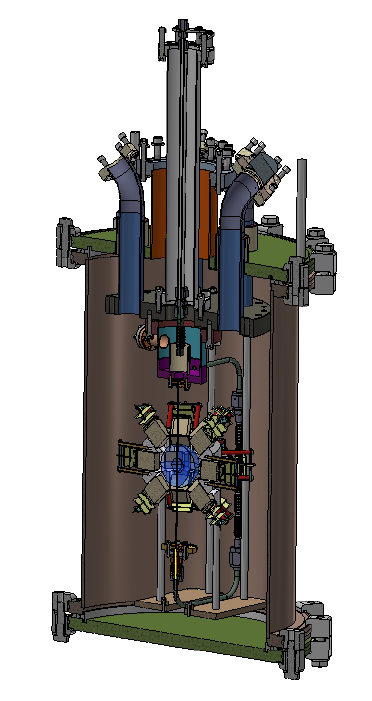
\includegraphics[width=0.75\textwidth , height=0.3\textheight]{detCAD.png}% Here is how to import 
	\end{subfigure}	
	\begin{subfigure}[b]{0.45\textwidth}
		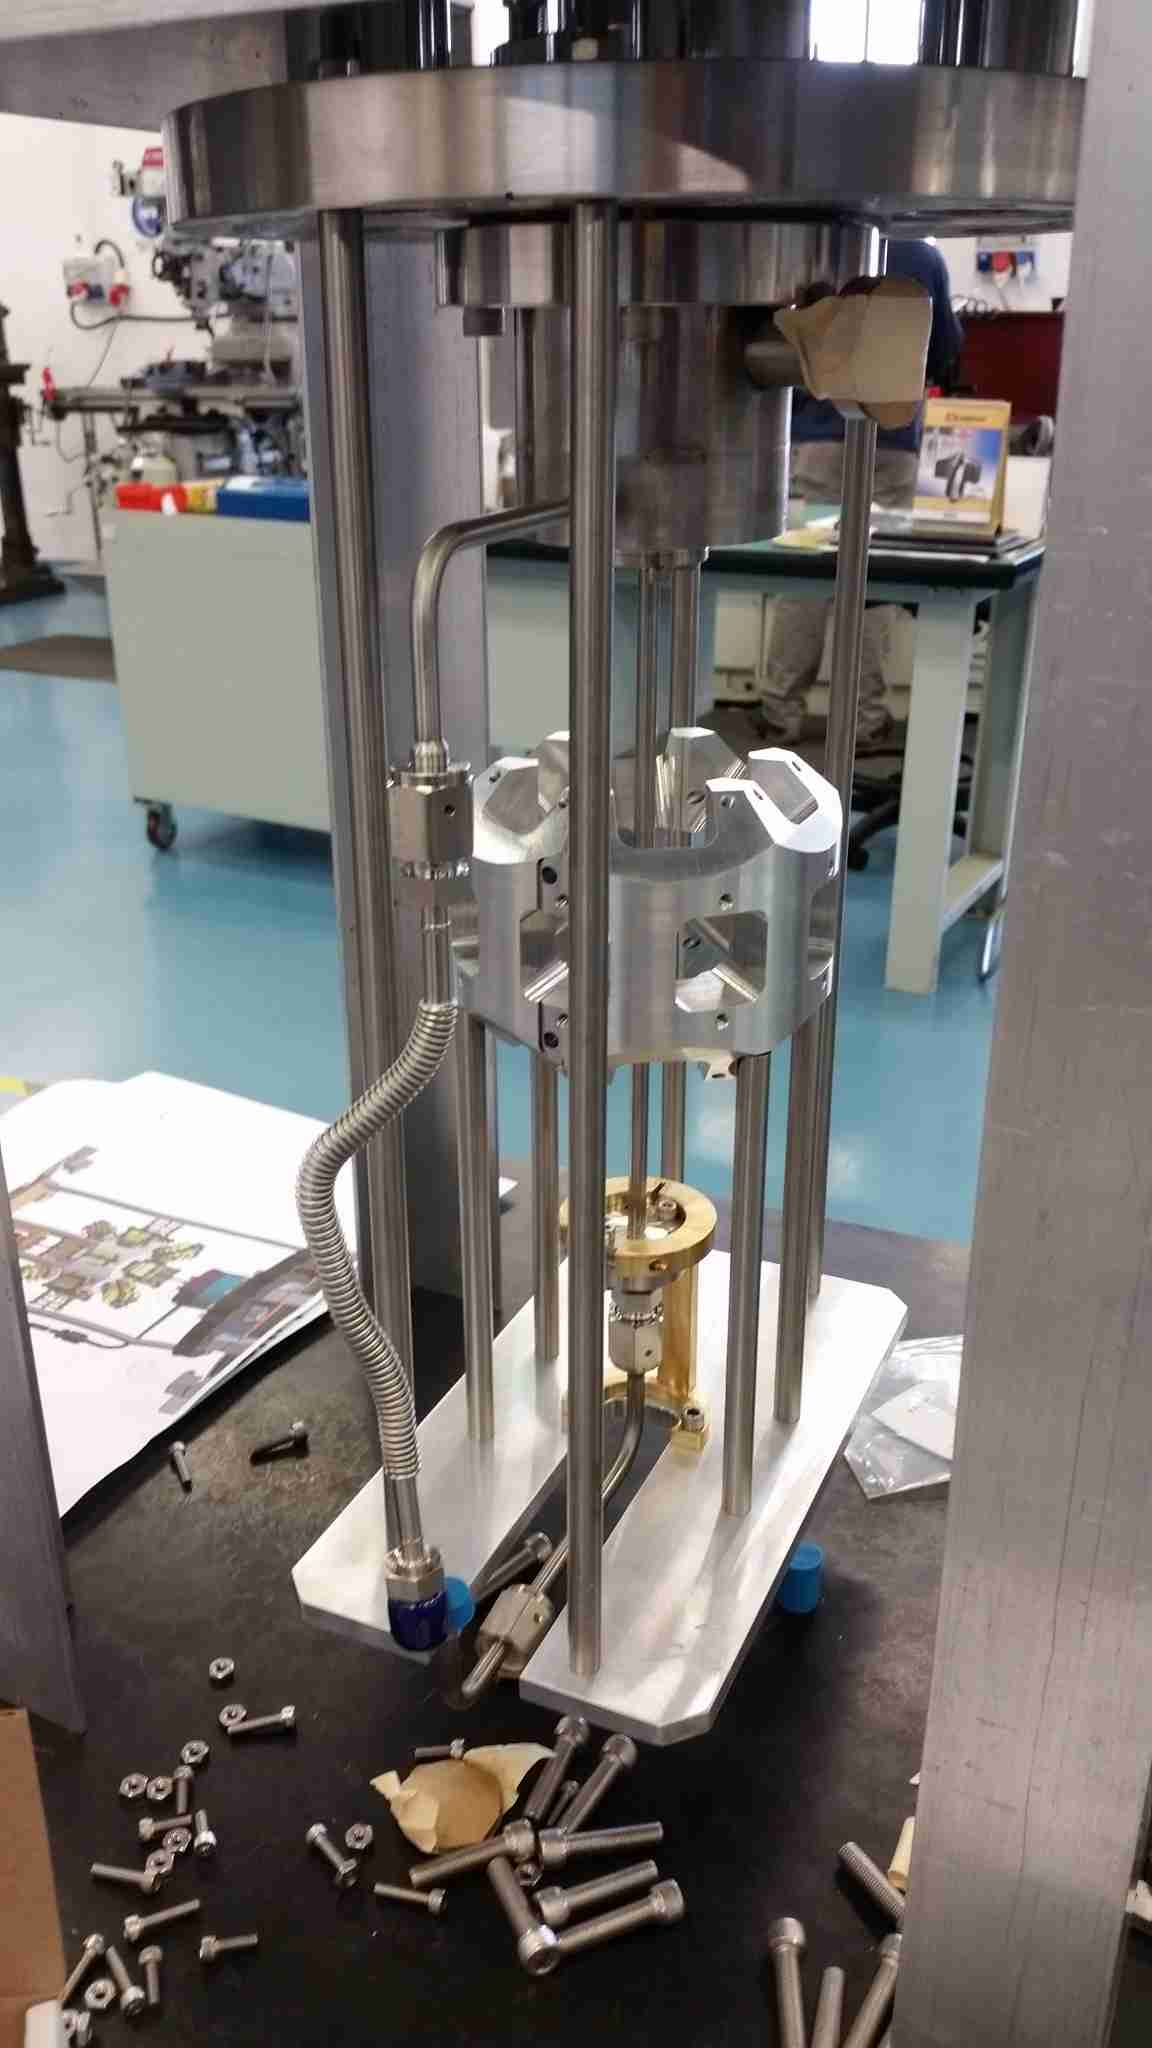
\includegraphics[width=\textwidth , height=0.3\textheight]{detReal_small.jpg}% Here is how to import 
	\end{subfigure}	
		\caption{\label{fig:detector} (Left) CAD design of the detector part. (Right) First mounting of the 
		detector part, still not connected to the rest of the system.}
	
\end{figure}
%%%%%%%%%%%%%%%%%%%%%%%%%%%%%%%%%%%%%%%%%%%%%%%%%%%%%%%%%%%%%%%%%%%%%%%%%%%%

\section{The DAQ System }
\label{sec:DAQ}

%%%%%%%%%%%%%%%%%%%%%%%%%%%%%%%%%%%%%%%%%%%%%%%%%%%%%%%%%%%%%%%%%%%%%%%%%%%%%%%%%%%%
%by MMdevi. Last modified July 2, 2017.
%%%%%%%%%%%%%%%%%%%%%%%%%%%%%%%%%%%%%%%%%%%%%%%%%%%%%%%%%%%%%%%%%%%%%%%%%%%%%%%%%%%%

The DAQ system consists of a heterogeneous system with both 
NIM and VME electronics modules, with the data readout being carried out 
through an optical link via a VME controller\footnote{CAEN V2718} and a 
PCIe card \footnote{CAEN A3818}. 

The schematic layout of the DAQ system is shown in Fig.~{\ref{Fig:DAQscheme}}. 
The PMTs are ramped up to +800V (the maximum is +900V) using a 24 channel VME high 
The raw electrical pulse output of the PMTs are denoted as S{\it i}(raw), where {\it i} = 1 -- 20. 
These raw pulses are then amplified and shaped using two photomultiplier preamplifiers 
\footnote{Phillips 776. 16 independent and direct-coupled amplifiers channels}. 
The preamplifier channels operates from DC to 275 MHz and produce two identical 
50 $\Omega$ non inverting FIFO outputs with voltage gains of 10. 
The amplified pulses are denoted as S{\it i} 
[\RanComment{Isn't this the same notation as the raw data?} \mmd{raw: S{\it i}(raw), amplified: S{\it i}. 
I specifically want to include 'raw' in the terms and a super/sub script would be unreadable in the schematic}], 
({\it i} = 1 -- 20). One of the two FIFO outputs from each channel is converted to a 
digital signal with an Analog to Digitizer converter \footnote{CAEN ADC V1742: Switched capacitor Digitizer}. 

%%%%%%%%%%%%%%%%%%%%%%%%%%%%%%%%%%%%%%%%%%%%%%%%%%%%%%%%%%%%%%%%%%%%%%%%%%
\begin{figure}[h]
   \centering
   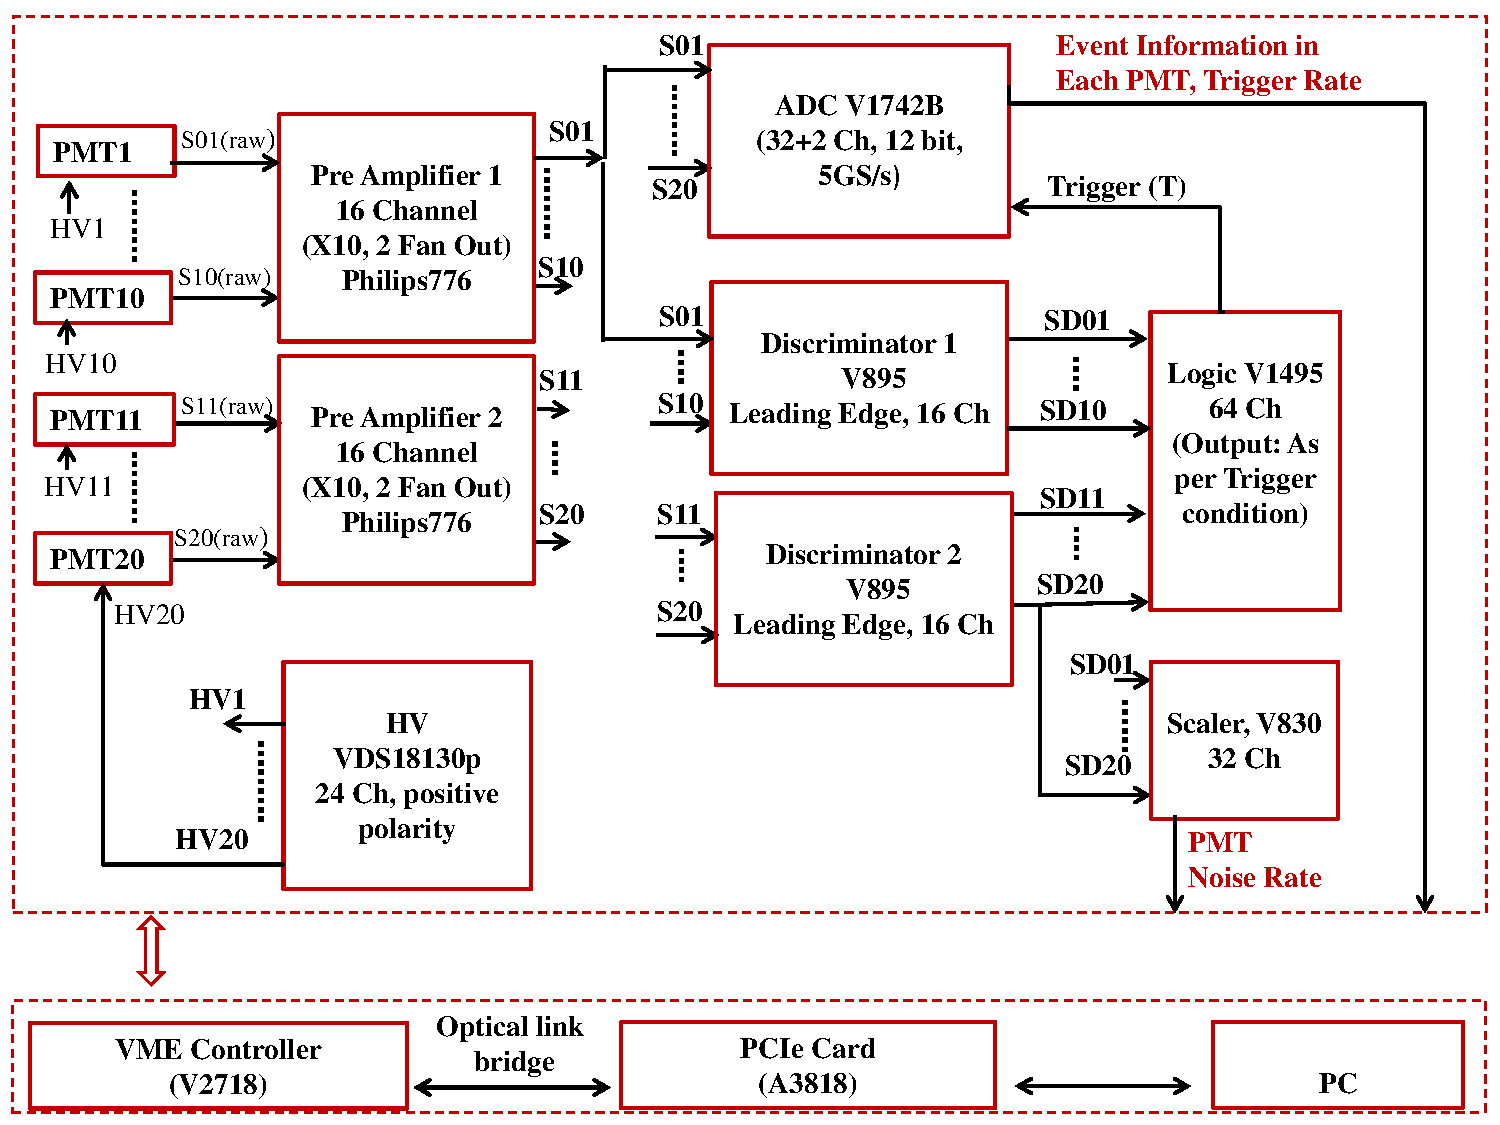
\includegraphics[width=0.85\textwidth]{DAQscheme.pdf}
   \caption{The schematic of the Data Acquisition System of DIREXENO. It 
        consists of 20 PMTs and the subsequent electronic channels to record 
        the events for an internal trigger generated by the coincidence of any 
        two PMTs in the system and also the PMT noise rate.}
   \label{Fig:DAQscheme}
\end{figure}
%%%%%%%%%%%%%%%%%%%%%%%%%%%%%%%%%%%%%%%%%%%%%%%%%%%%%%%%%%%%%%%%%%%%%%%%%%%

The schematic layout 
of the DAQ system is shown in Fig.~{\ref{Fig:DAQscheme}}. All the 20 PMTs 
are oriented in the holder assembly which was discussed in section \ref{subsubsec:sphere}. 
The PMTs are ramped up to +800V (the maximum is +900V) using a 24 channel 
VME high voltage distributor module \footnote{iseg VDS18130p : 24 independent channels with positive polarity}.  
The raw electrical pulse output of the PMTs are defined as S{\it i} (raw), where {\it i} = 1 -- 20. 
These raw pulses are then 
amplified and shaped using two photomultiplier preamplifiers \footnote{Phillips 776: 16 independent  and direct-coupled 
amplifiers channels}. The preamplifier channels operates from DC to 275 MHz and 
produce two identical 50 $\Omega$ non inverting outputs with voltage gains of 10. 
The amplified pulses as defined as S{\it i}, ({\it i} = 1 -- 20). One out of the 
two identical analog outputs from each channel is converted to a digital 
signal with an Analog to Digitizer converter \footnote{CAEN ADC V1742: 
32 channel switched capacitor Digitizer}. 


The ADC consists of two 12bit 5GS/s Switched capacitor Digitizer sections, 
each of them with 16+1 channels, based on DRS4 chip. The dynamic range of the input signal is 1 
Vpp with adjustable DC offset. This module can sample either bipolar or unipolar analog input 
signal within the dynamic range in a circular 
analog memory buffer, with default sampling frequency choices 5GS/s, 2.5 GS/s 
or 2 GS/s. As soon as a trigger signal reaches, all the analog memory 
buffers gets frozen and then gets digitized into a digital memory buffer 
with a 12 bit resolution. 

An intrinsic trigger is generated for the system, 
with the coincidence of any two out of the twenty PMTs. The second output from the 
preamplifier channels are converted to binary signals using two 16 channel leading 
Edge discriminator \footnote{CAEN V895}. In Fig.~\ref{Fig:DAQscheme}, the binary 
outputs from the discriminator are denoted as SD{\it i}, i= 1 -- 20. The SD{\it i} signals are then passed over to 
the logic module \footnote{CAEN V1495: FPGA based General purpose VME board} to obtain the trigger. The output of the logic operation is 
used to trigger the ADC. In order to record the PMT noise rate, the 
SD{\it i} signals are duplicated and fed to a scaler \footnote{CAEN V830: 16 channel}.

The PMT event information and the trigger rate are read from the ADC, while the Scaler 
records the PMT noise rate. The further analyses of the 
relevant events in the PMTs are carried out offline using an analysis 
framework.










%\clearpage %temporary TBC

\section{Optical properties of the sphere }
\label{sec:opt}

The central component of the experiment is the HPFS sphere, which holds the LXe target, located in the center 
of the detector system. The sphere is made of two Corning HPFS 8655 hemispheres attached by a UV transparent glue. 
The refractive index of this HPFS is 1.58 at 185 nm, matching to the LXe one, which is 1.61. Hence, there is minimal 
diffraction from the original direction of the photons as they transit from the LXe target to the sphere. The refractive 
indexes at various wavelengths are shown in Fig.~\ref{fig:hpfsRIcalibration} (left panel).


<<<<<<< HEAD
The HPFS transparency to VUV photons is an extremely crucial parameter for setting the sphere's dimensions (inner and outer radii). 
Therefore, the transmittance of an HPFS sample was measured, using a VUV monochromator light source. 
The measured transmittances as a function of wavelength are shown in Fig.~\ref{fig:hpfsRIcalibration}~(right panel). The 
transmittance of the sample at 178~\,nm, is$\sim98.7$\,\%/cm.  
=======
The HPFS transparency to VUV photons is an extremely crucial parameter for setting the sphere's dimensions (inner and outer radii) and detector sensitivity. Therefore, the transmittance of an HPFS sample was measured, using a VUV monochromator light source. 
The measured transmittances as a function of wavelength are shown in Fig.~\ref{fig:hpfsRIcalibration}~(right panel). The \sout{intrinsic} transmittance of the sample at 178~\,nm, is$\sim98.7$\,\%/cm.  
>>>>>>> 2292d93adb63079752489fa3b355837dcdd54054

\begin{figure}[h]
   \centering
   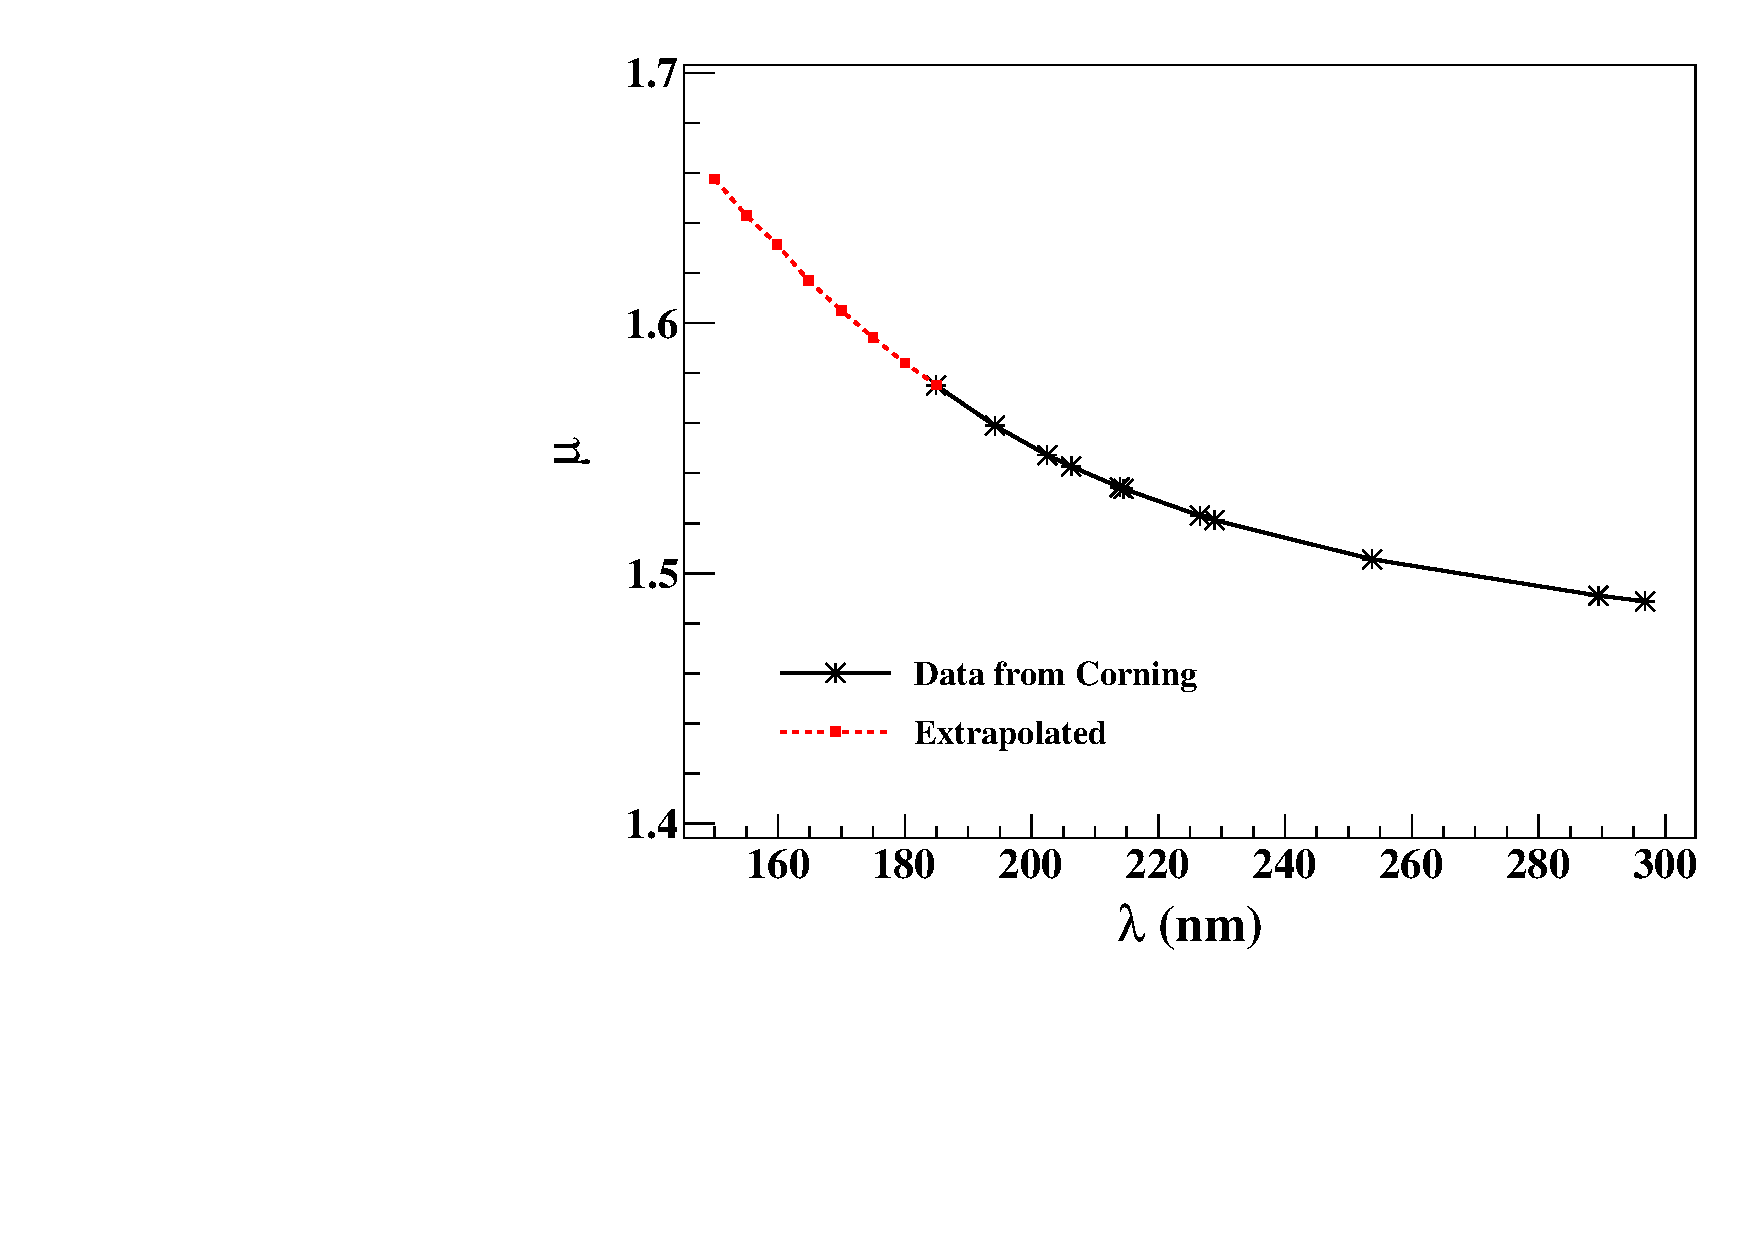
\includegraphics[width=0.48\textwidth]{RI-calibration.pdf}
    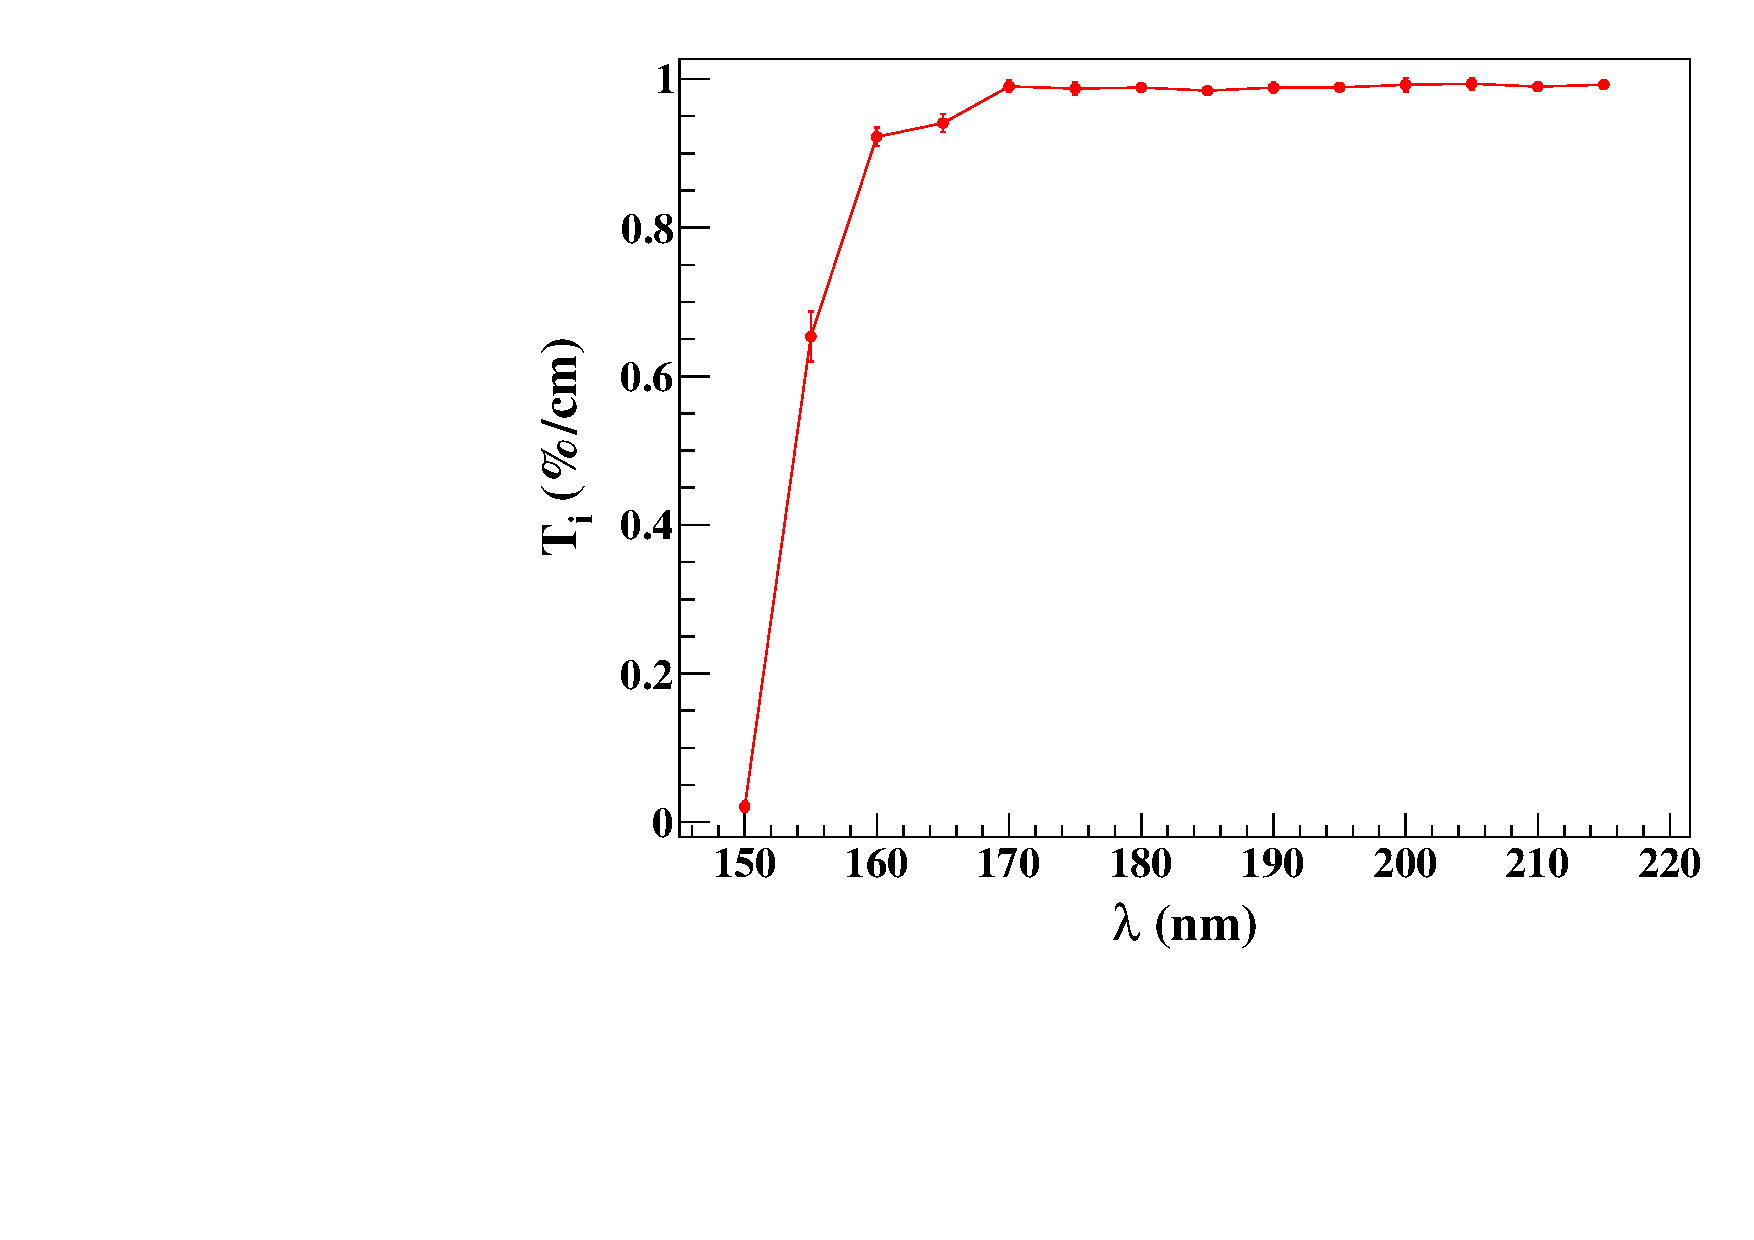
\includegraphics[width=0.48\textwidth]{IntTransmittance.pdf}
   \caption{Some relevant characteristics of HPFS-8655. (Left) The refractive index as provided by corning and 
   extrapolated to relevant wavelength range. (Right) The internal transmittance ($T_{i}$).} 
   \label{fig:hpfsRIcalibration}
\end{figure}


The shell should be thick enough to reduce internal reflections, but not 
<<<<<<< HEAD
too thick to attenuate the scintillation light and the LXe target bubble within it should not be too large in order to avoid double scatters. 
The sources that will be used for exciting the xenon, and creating the supperradiance 
=======
too thick to attenuate the scintillation light. The LXe target bubble within should not be too large in order to avoid double scatters. The sources that will be used for exciting the xenon, and creating the supperradiance 
>>>>>>> 2292d93adb63079752489fa3b355837dcdd54054
(signal) as well as the standard emission (background), will be $^{137} \mathrm{Cs}$ 
(E$_\gamma$=662 keV) and $^{57} \mathrm{Co}$( E$_\gamma$= 122keV \& 136 keV) for ER with mean free path of $\sim4$\,cm and $\sim1$\,cm respectively. For NR $^{241}$AmBe , 
D-D neutron generator, or neutron produced in an accelerator will be used.

Using a GEANT4 based simulation~\cite{AGOSTINELLI2003250} studying the path of the scintillation photons the sphere dimensions are optimized. 
The outer radius  is 3 cm, and the inner (the hollow space that holds the LXe) is 1 cm. 

\section{Simulation (\mmd{in progress})}
\label{sec:sim}
%%%%%%%%%%%%%%%%%%%%%%%%%%%%%%%%%%%%%%%%%%%%%%%%%%%%%%%%%%%%%%%%%%%%%%%%%%%%%%%%%%%%%%%%%%%%%%%%%%%%%%%%%%%%%%%%%%%%%%%%
To asses the sensitivity of the detector to identify an emission pattern a GEANT4 based simulation is used. 
Several emission types and the propagation of photons in the detector are simulated to produce the hit patern  
at the PMTs for each type. 
Assuming a number of test patterns of the LXe scintillation, the photons detected at the PMTs are mapped and put 
through a statistical test to check the detector's sensitivity towards those patterns.

The realistic dimension of the detector assembly is used in the simulation. The important 
geometrical and optical parameters are listed in Table~\ref{tab:OptPar}. 
The probability for a photon being transmitted/reflected at a given surface is 
determined by Fresnel's equations, which include Snell's law for the transmitted light, 
and specular reflection for the reflected light. The boundary surfaces between different media
such as, the LXe--HPFS, HPFS--vacuum and vacuum--PMT, are assumed to be perfectly smooth, 
therefore enabling only specular reflection.

%%%%%%%%%%%%%%%%%%%%%%%%%%%%%%%%%%%%%%%%%%%%%%%%%%%%%%%%%%%%%%%%%%%%%%%%%%%%%%%%%%%%%%%
\begin{table}[h]
  \centering
  \caption{The parameters used in simulation}
  \label{tab:OptPar}
  \begin{tabular}{|c c||c c|}
  \hline
  Parameter & Value & Parameter & Value \\
  \hline
  LXe absorption length & 100 cm & No. of PMT & 20\\
  %\hline
  LXe scattering length & 35 cm & PMT active area & 22mm $\times$ 22mm\\
  %\hline
  HPFS absorption length & 100 cm & PMT QE & $\geq$ 30\% \\
 % \hline
  HPFS scattering length & $\infty$ & PMT distance from centre & 39 mm\\
 % \hline
  LXe refractive index & 1.61 & LXe bubble radius & 1cm\\
  %\hline
  HPFS refractive index & 1.57 & HPFS shell thickness & 2 cm \\
  Scintillation wavelength & 178 $\pm$ 14 nm & Invar tube diameter & 1 mm\\
  \hline
 \end{tabular}
\end{table}
%%%%%%%%%%%%%%%%%%%%%%%%%%%%%%%%%%%%%%%%%%%%%%%%%%%%%%%%%%%%%%%%%%%%%%%%%%%%%%%%%%%%%%%

The photons reaching the PMTs can either be detected, absorbed or reflected from the photocathode 
or the PMT window. A simplified approach of the above possibilities is considered -- 
A photon on the PMT has 30\% probability to be detected (since QE $\geq$ 30\%), 50\% probability to get 
absorbed and 20\% probability to get specularly reflected. As the scintillation light in a particular 
event is emitted by a cloud of excited diatomic molecules, with a linear size much smaller than that 
of the optical system, each event is simulated as a number of photons that are emitted from a point 
in the LXe. The events are uniformly generated in the LXe volume to simulate an entirely radiated 
target much smaller than the mean free path length of the source particles in LXe.

For each scintillation event, a number of photons are detected by the PMTs, with a possibility of 
no photons detected by some of the PMTs. The exact position on the photocathode which the photons hit, 
and the exact number of photons falling on a PMT are not known. The electronic signal generated in a PMT 
for a certain number of incident photon is statistical in nature. The simulation is performed for both 
ideal photon counting and statistical photon counting. The R8520 PMTs also has  ~20\% probability 
for double photoelectris emission for 178 nm photons, which is also included in the simulation.
Each detected photon 
on a PMT is then assigned a uniformly random position on the PMT surface. The direction of this point with respect 
to the center of the LXe sphere is defined as the incident direction of the photon. The direction information 
is then used to calculate the angles between all possible pairs of photon in an event.

In order to test the emission pattern, the angle correlation distribution of a large sample ($10^5$ events) 
from isotropic emission is considered to be the PDF of the null hypothesis and is compared 
to that of a number of smaller samples ($10^4$ events) from different types of anisotropic emissions. 
The reduced $\chi^2$ for each sample is calculated as follows.

\begin{equation}
\chi^2/\nu = \frac{1}{\nu} \sum^{\nu}_{i=1} \frac{(O_i - E_i)^2}{E_i}
\label{redchi2}
\end{equation}

where, $O_i$ is the observed count in the $i^{th}$ angle bin, $E_i$ is the expected count in the $i^{th}$ 
angle bin and $\nu$ is the total number of angle bins which is also the degree of freedom. In this analysis, 
60 bins of identical width are used. The anisotropic emission patterns used in the analysis are listed 
in Table~\ref{tab:AnisoPattern}. For each emission pattern,  an anisotropic pattern is taken to be embedded 
in an isotropic background. The fraction of photons in the anisotropic pattern ($r_{aniso}$) is 10 \% of the net photons 
and the rest is the isotropic background. For multiple beams in a pattern $r_{aniso}$ is spitted among them 
as mentioned in the Table. The intensity of the beams of photons are of Gaussian nature, and their emission direction are 
randomly varied in each event.

%%%%%%%%%%%%%%%%%%%%%%%%%%%%%%%%%%%%%%%%%%%%%%%%%%%%%%%%%%%%%%%%%%%%%%%%%%%%%%%%%%%%%%%
\begin{table}[h]
  \centering
  \caption{Emission patterns. For all patterns $r_{aniso}$ = 0.1 from a 
  total of 50 photon/event.}
  \label{tab:AnisoPattern}
  \begin{tabular}{|c | c| c | c|}
  \hline
  Pattern no. & No. of beams and type & Beam half widths & Signal fractions \\
  %\hline
  1 & 1 & $\sigma_1$ = $5^{0}$ & $r_1$ = 1 \\
  %\hline
   2 & 1 & $\sigma_1$ = $15^{0}$ & $r_1$ = 1 \\
  %\hline
   3 & 2 correlated & $\sigma_1$ = $5^{0}$, $\sigma_2$ = $5^{0}$ & $r_1$ = 0.5, $r_2$ = 0.5  \\
  %\hline
   4 & 2 correlated & $\sigma_1$ = $15^{0}$, $\sigma_2$ = $15^{0}$ & $r_1$ = 0.5, $r_2$ = 0.5 \\
  %\hline
   5 & 2 correlated & $\sigma_1$ = $5^{0}$, $\sigma_2$ = $10^{0}$ & $r_1$ = 0.5, $r_2$ = 0.5 \\
  %\hline
   6 & 2 correlated & $\sigma_1$ = $30^{0}$, $\sigma_2$ = $10^{0}$ & $r_1$ = 0.5, $r_2$ = 0.5 \\
  %\hline
   7 & 2 correlated & $\sigma_1$ = $5^{0}$, $\sigma_2$ = $5^{0}$ & $r_1$ = 0.5, $r_2$ = 0.5 \\
  %\hline
   8 & 2 correlated & $\sigma_1$ = $15^{0}$, $\sigma_2$ = $15^{0}$ & $r_1$ = 0.5, $r_2$ = 0.5 \\
  %\hline
   9 & 2 correlated & $\sigma_1$ = $10^{0}$, $\sigma_2$ = $30^{0}$ & $r_1$ = 0.2, $r_2$ = 0.8 \\
  %\hline
    10 & 2 correlated & $\sigma_1$ = $30^{0}$, $\sigma_2$ = $10^{0}$ & $r_1$ = 0.2, $r_2$ = 0.8 \\
  \hline
 \end{tabular}
\end{table}
%%%%%%%%%%%%%%%%%%%%%%%%%%%%%%%%%%%%%%%%%%%%%%%%%%%%%%%%%%%%%%%%%%%%%%%%%%%%%%%%%%%%%%%

Results:

%%%%%%%%%%%%%%%%%%%%%%%%%%%%%%%%%%%%%%%%%%%%%%%%%%%%%%%%%%%%%%%%%%%%%%%%%
\begin{figure}[h]
\centerline{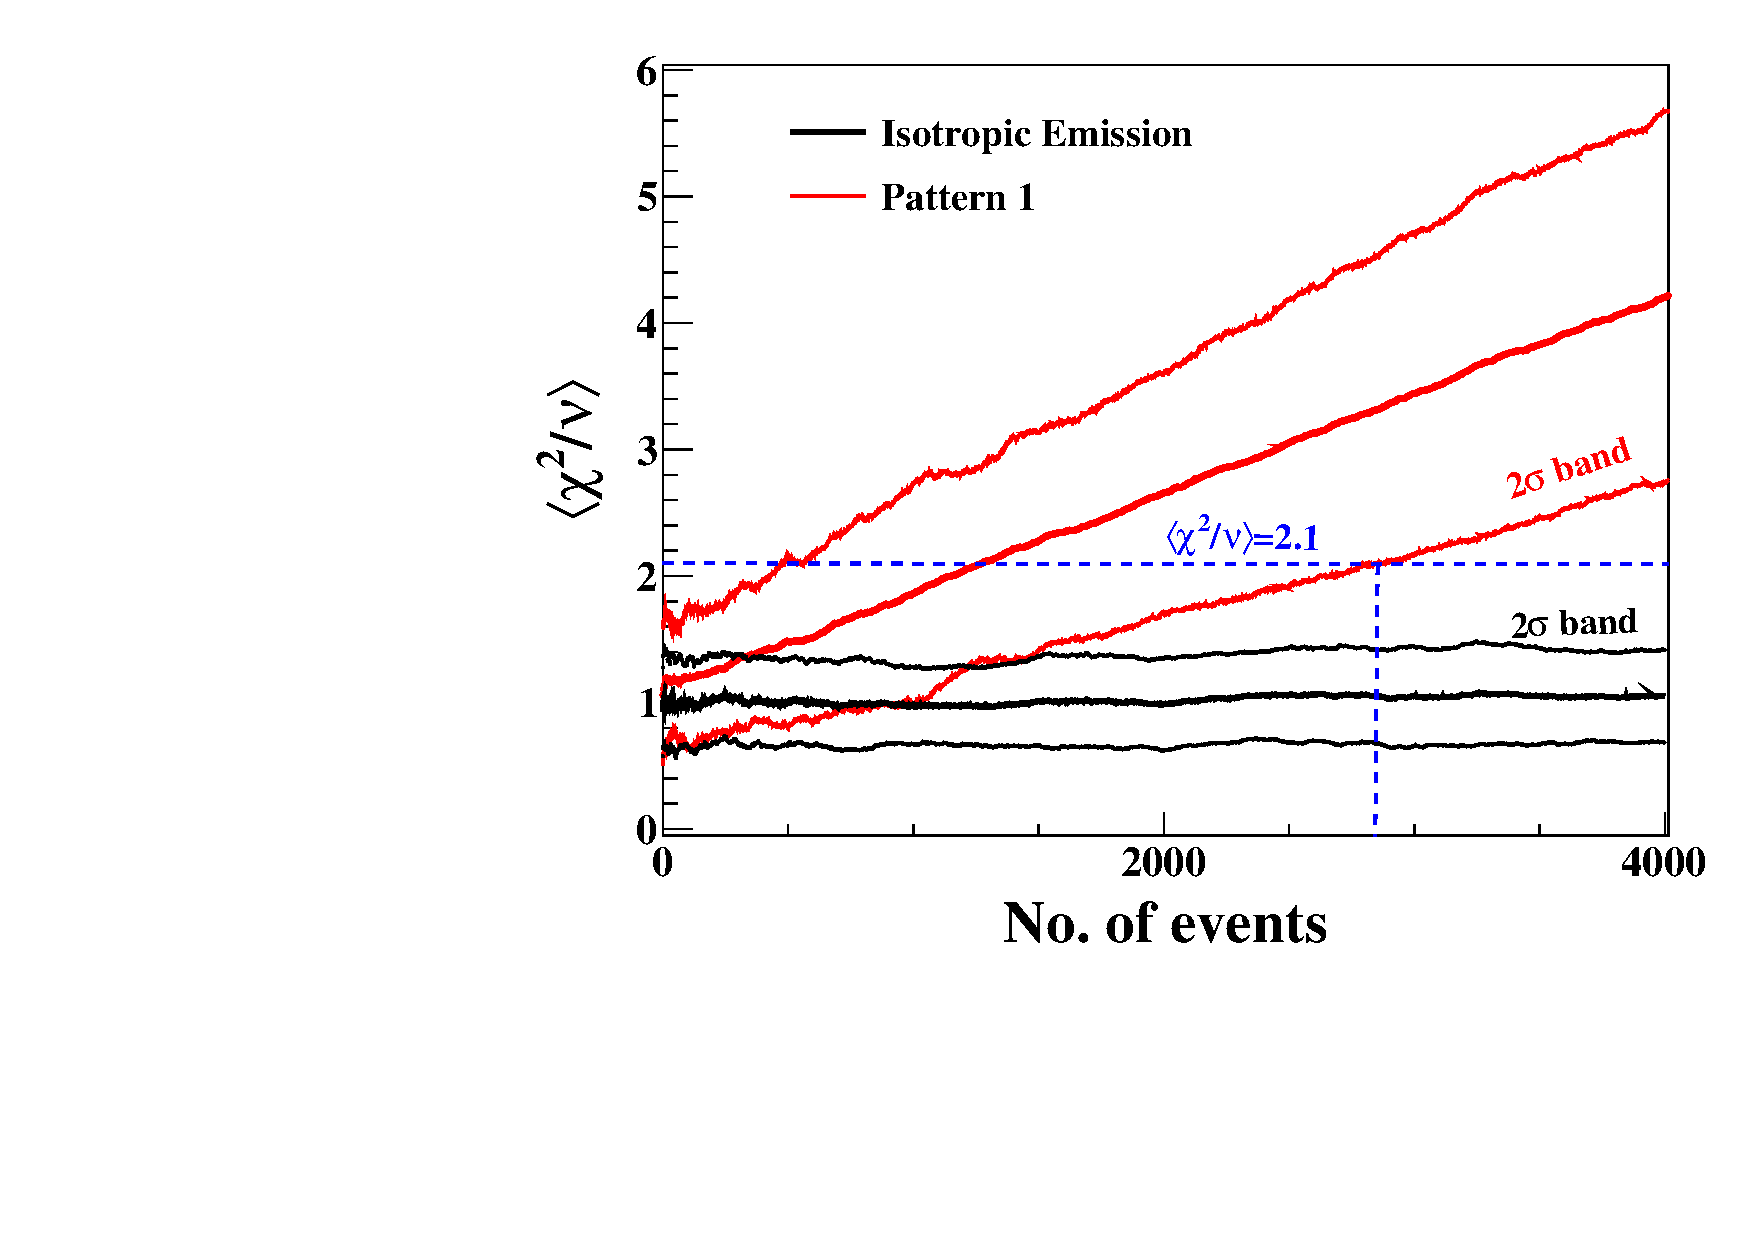
\includegraphics[width=0.5\linewidth]{Pattern1.pdf}}
\caption{}
\label{fig:pattern1}
\end{figure}
%%%%%%%%%%%%%%%%%%%%%%%%%%%%%%%%%%%%%%%%%%%%%%%%%%%%%%%%%%%%%%%%%%%%%%%%%%%%

\section{Summary}
\label{sec:summary}

The setup of Direxeno, an experiment to measure the spatial and temporal distribution of LXe scintillation, has 
been presented. The system consists of 4 main building blocks (gas handling, cryogenic, detector, 
and DAQ), each of which can be exchanged without altering others allowing significant flexibility 
and modularity. Each of the building blocks has been described in detail, with emphasis on the design 
and components.

The sensitivity of the setup to different postulated non isotropic emission patterns are studied using MC simulations. For the patterns studied, a run--time of 2-3 weeks is required using typical radioactive 
sources. Therefore the system is designed to maintain stability over a reasonable time period.

Using DireXeno, effects like superradiance or any other non-linear scintillation can be measured. 
Measuring the correlation between the direction of the emission and the direction of the radioactive 
source, may lead to directionality measurement which will allow enhanced statistical modeling of 
background and improved sensitivity in DM experiments.



%%% BIBLIOGRAPHY %%%

%\bibliographystyle{apsrev}
\bibliographystyle{unsrt}
\bibliography{DirexenoBib}

\end{document}
\grid
